\documentclass[10pt,twocolumn]{article}
\usepackage[margin=2.5cm]{geometry}
\usepackage{graphicx}
\usepackage{amsmath}
\usepackage{booktabs}
\usepackage{hyperref}
\usepackage{float}
\usepackage{caption}
\usepackage{subcaption}

\title{Student Dropout Prediction: A Machine Learning Analysis\\
\large DSAA2011 (L01) Course Project --- HKUST(GZ) 2026 Spring}
\author{
  [GroupID] \quad
  Member A (XX\%) \quad
  Member B (XX\%) \quad
  Member C (XX\%) \quad
  Member D (XX\%)
}
\date{\today}

\begin{document}
\maketitle

\begin{abstract}
We analyze the UCI Student Dropout and Academic Success dataset (4,424 samples, 36 features, 3 classes) using a complete machine learning pipeline encompassing data preprocessing, dimensionality reduction, clustering, supervised classification, and model evaluation. Our best-performing model achieves competitive F1-scores through hyperparameter tuning guided by validation curves. We find that academic performance features are the strongest predictors, and the ``Enrolled'' class is consistently the hardest to classify.
\end{abstract}

% ====================
\section{Introduction}

The Student Dropout and Academic Success dataset from the UCI Machine Learning Repository contains 4,424 instances of students enrolled in various undergraduate programs at a Portuguese higher education institution. Each instance is described by 36 features covering demographics, socioeconomic background, and academic performance across the first and second semesters. The classification target has three categories: \textbf{Dropout} (32.1\%), \textbf{Enrolled} (18.0\%), and \textbf{Graduate} (49.9\%).

Our objectives are: (1) explore data structure through visualization and clustering; (2) train and evaluate supervised classifiers; (3) improve models via validation-driven tuning; (4) investigate feature importance and ensemble methods.

% ====================
\section{Mandatory Tasks}

\subsection{Data Preprocessing}

We classified the 36 raw features into four types: \textit{nominal} (8 features, one-hot encoded), \textit{binary} (8 features, kept as 0/1), \textit{continuous} (7 features), and \textit{count} (13 features). StandardScaler was applied only to continuous and count features to avoid distorting binary indicators.

Feature engineering produced 22 additional domain features across six groups: academic ratios (approval rates, grade improvement), socioeconomic indicators, financial risk flags, demographic categories, macroeconomic indices, and application behavior features. Out-of-fold target encoding was used for high-cardinality categorical features to prevent data leakage.

The dataset was split 70/15/15 into training, validation, and test sets. Feature selection retained the top-50 features by tree-based importance (out of 61 candidates after target encoding).

\begin{figure}[H]
\centering
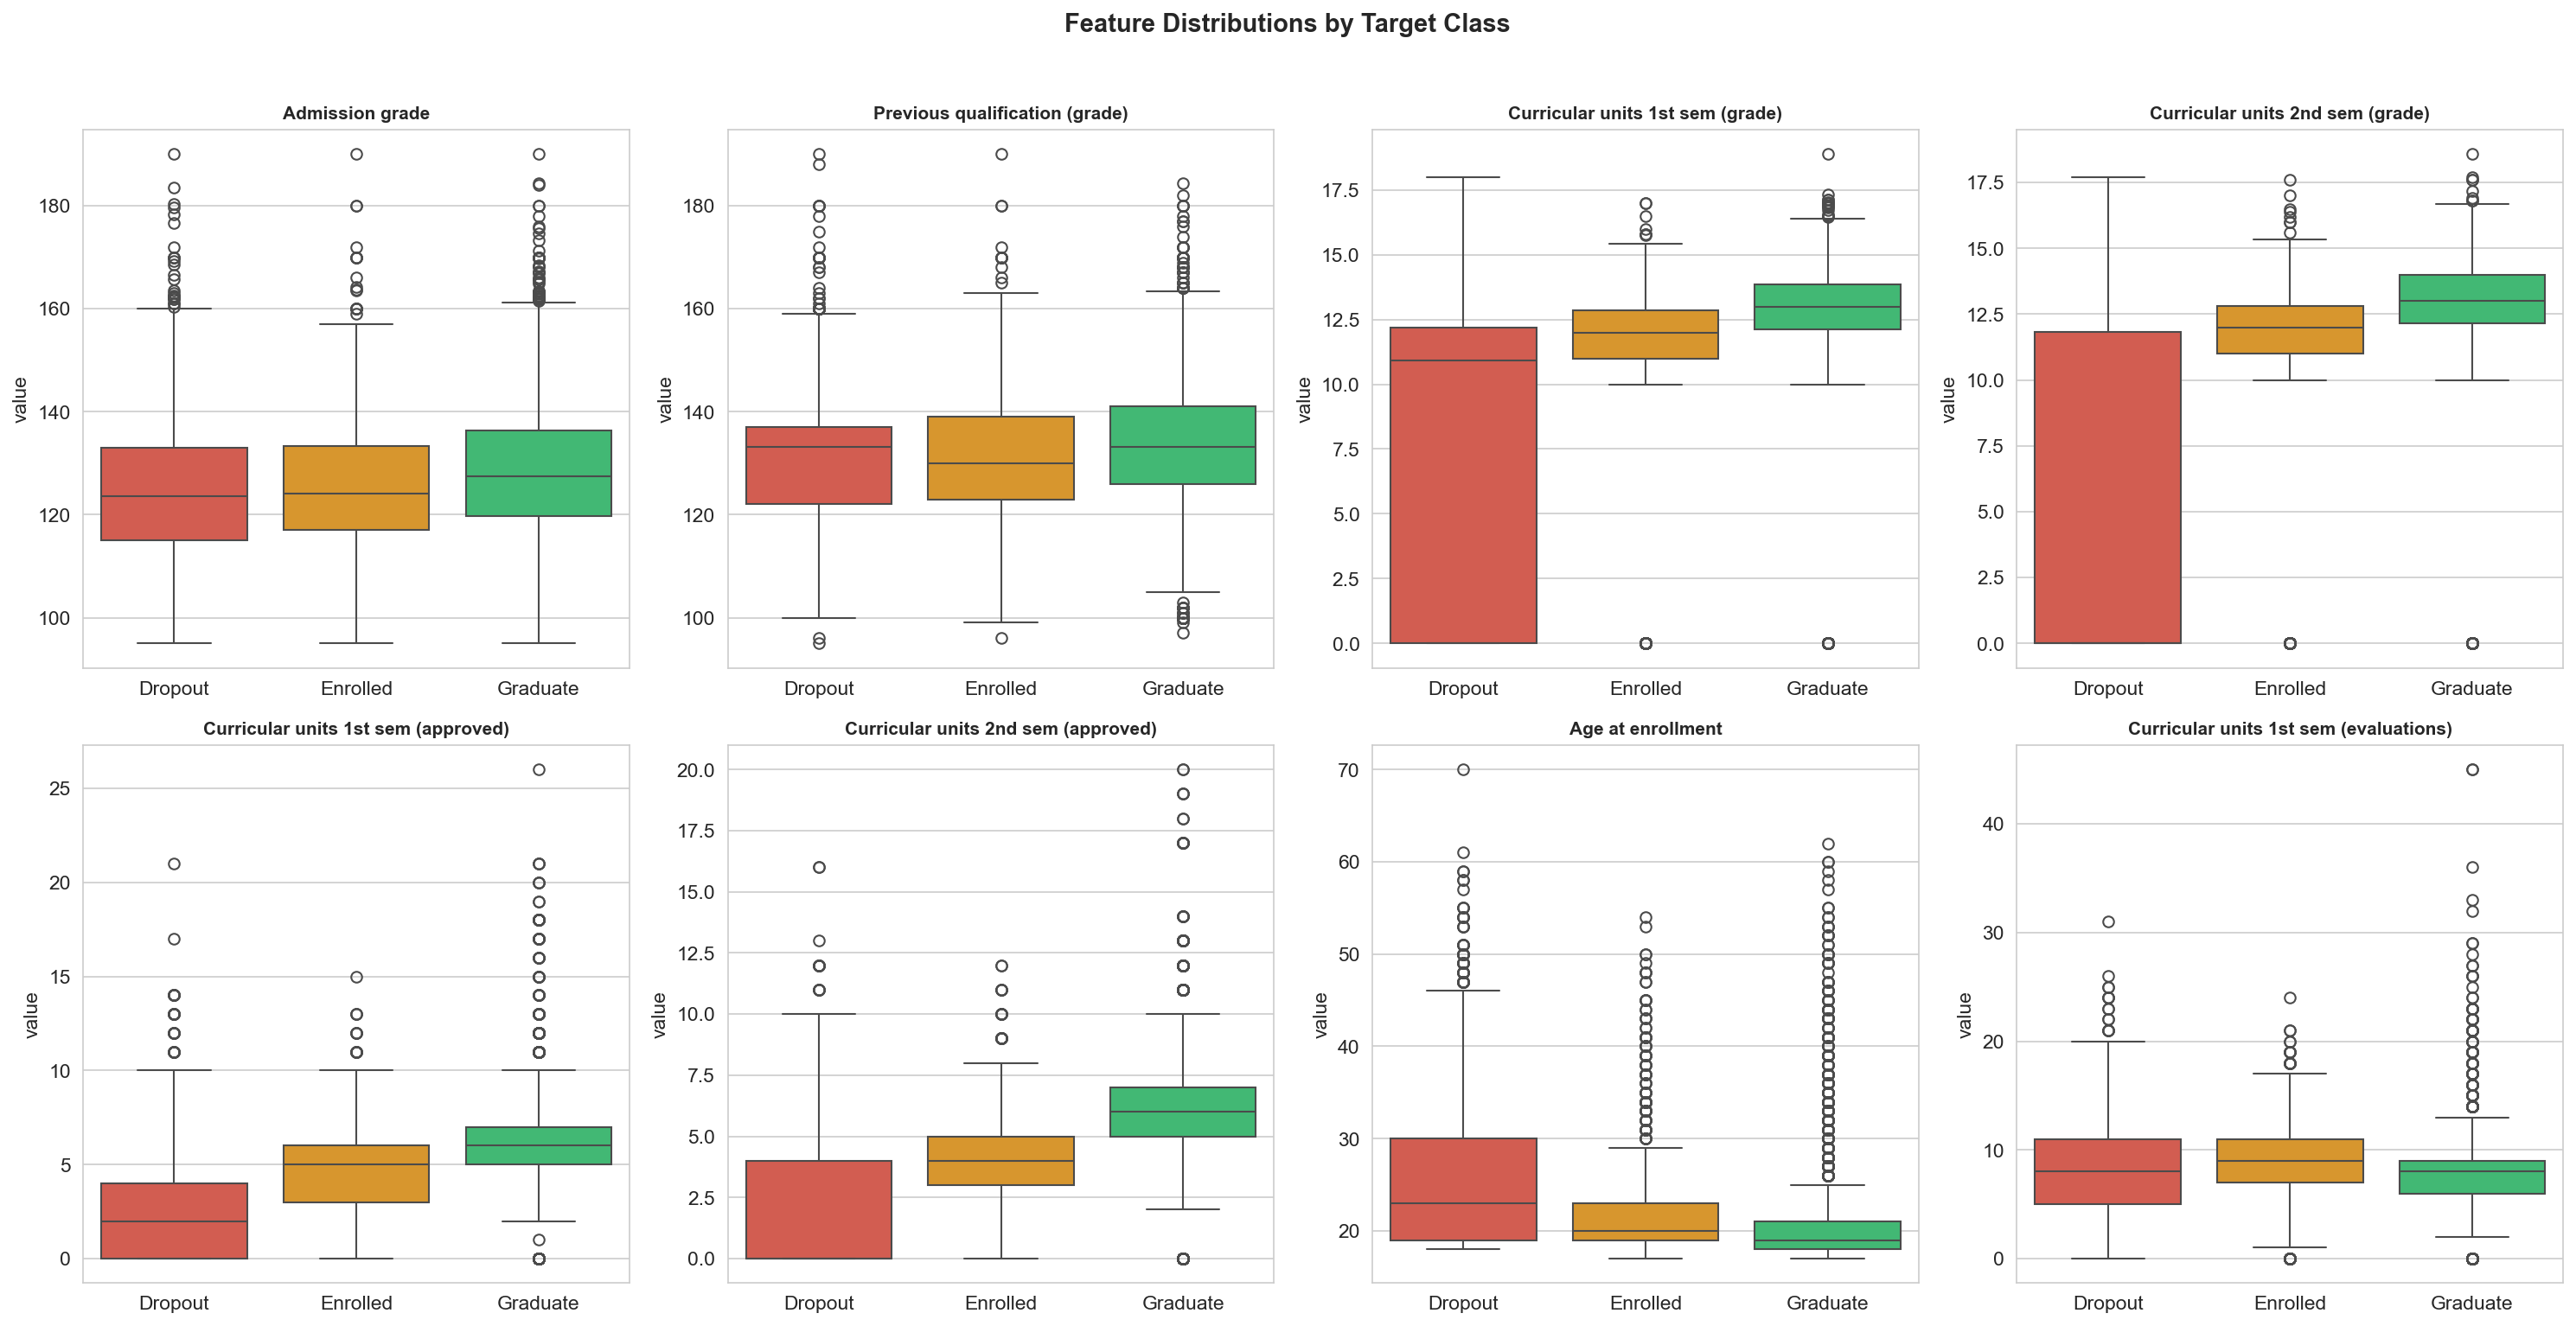
\includegraphics[width=\linewidth]{../data/plots/01_eda_boxplots.png}
\caption{Feature distributions by target class.}
\label{fig:eda_boxplots}
\end{figure}

\textbf{Missing values:} The dataset contains zero missing values across all 4,424 samples and 36 features, so no imputation was necessary.

\textbf{Exploratory Data Analysis (EDA)} reveals several key patterns (Figure~\ref{fig:eda_boxplots}): (1) Graduate students have notably higher 1st/2nd semester grades than Dropout students, while Admission grade shows less discrimination. (2) Dropout students tend to be older (higher median age at enrollment). (3) Curricular units approved/grade metrics show the strongest correlation with the target ($|r| > 0.3$). (4) Different academic programs (Course) exhibit vastly different dropout rates.

\begin{figure}[H]
\centering
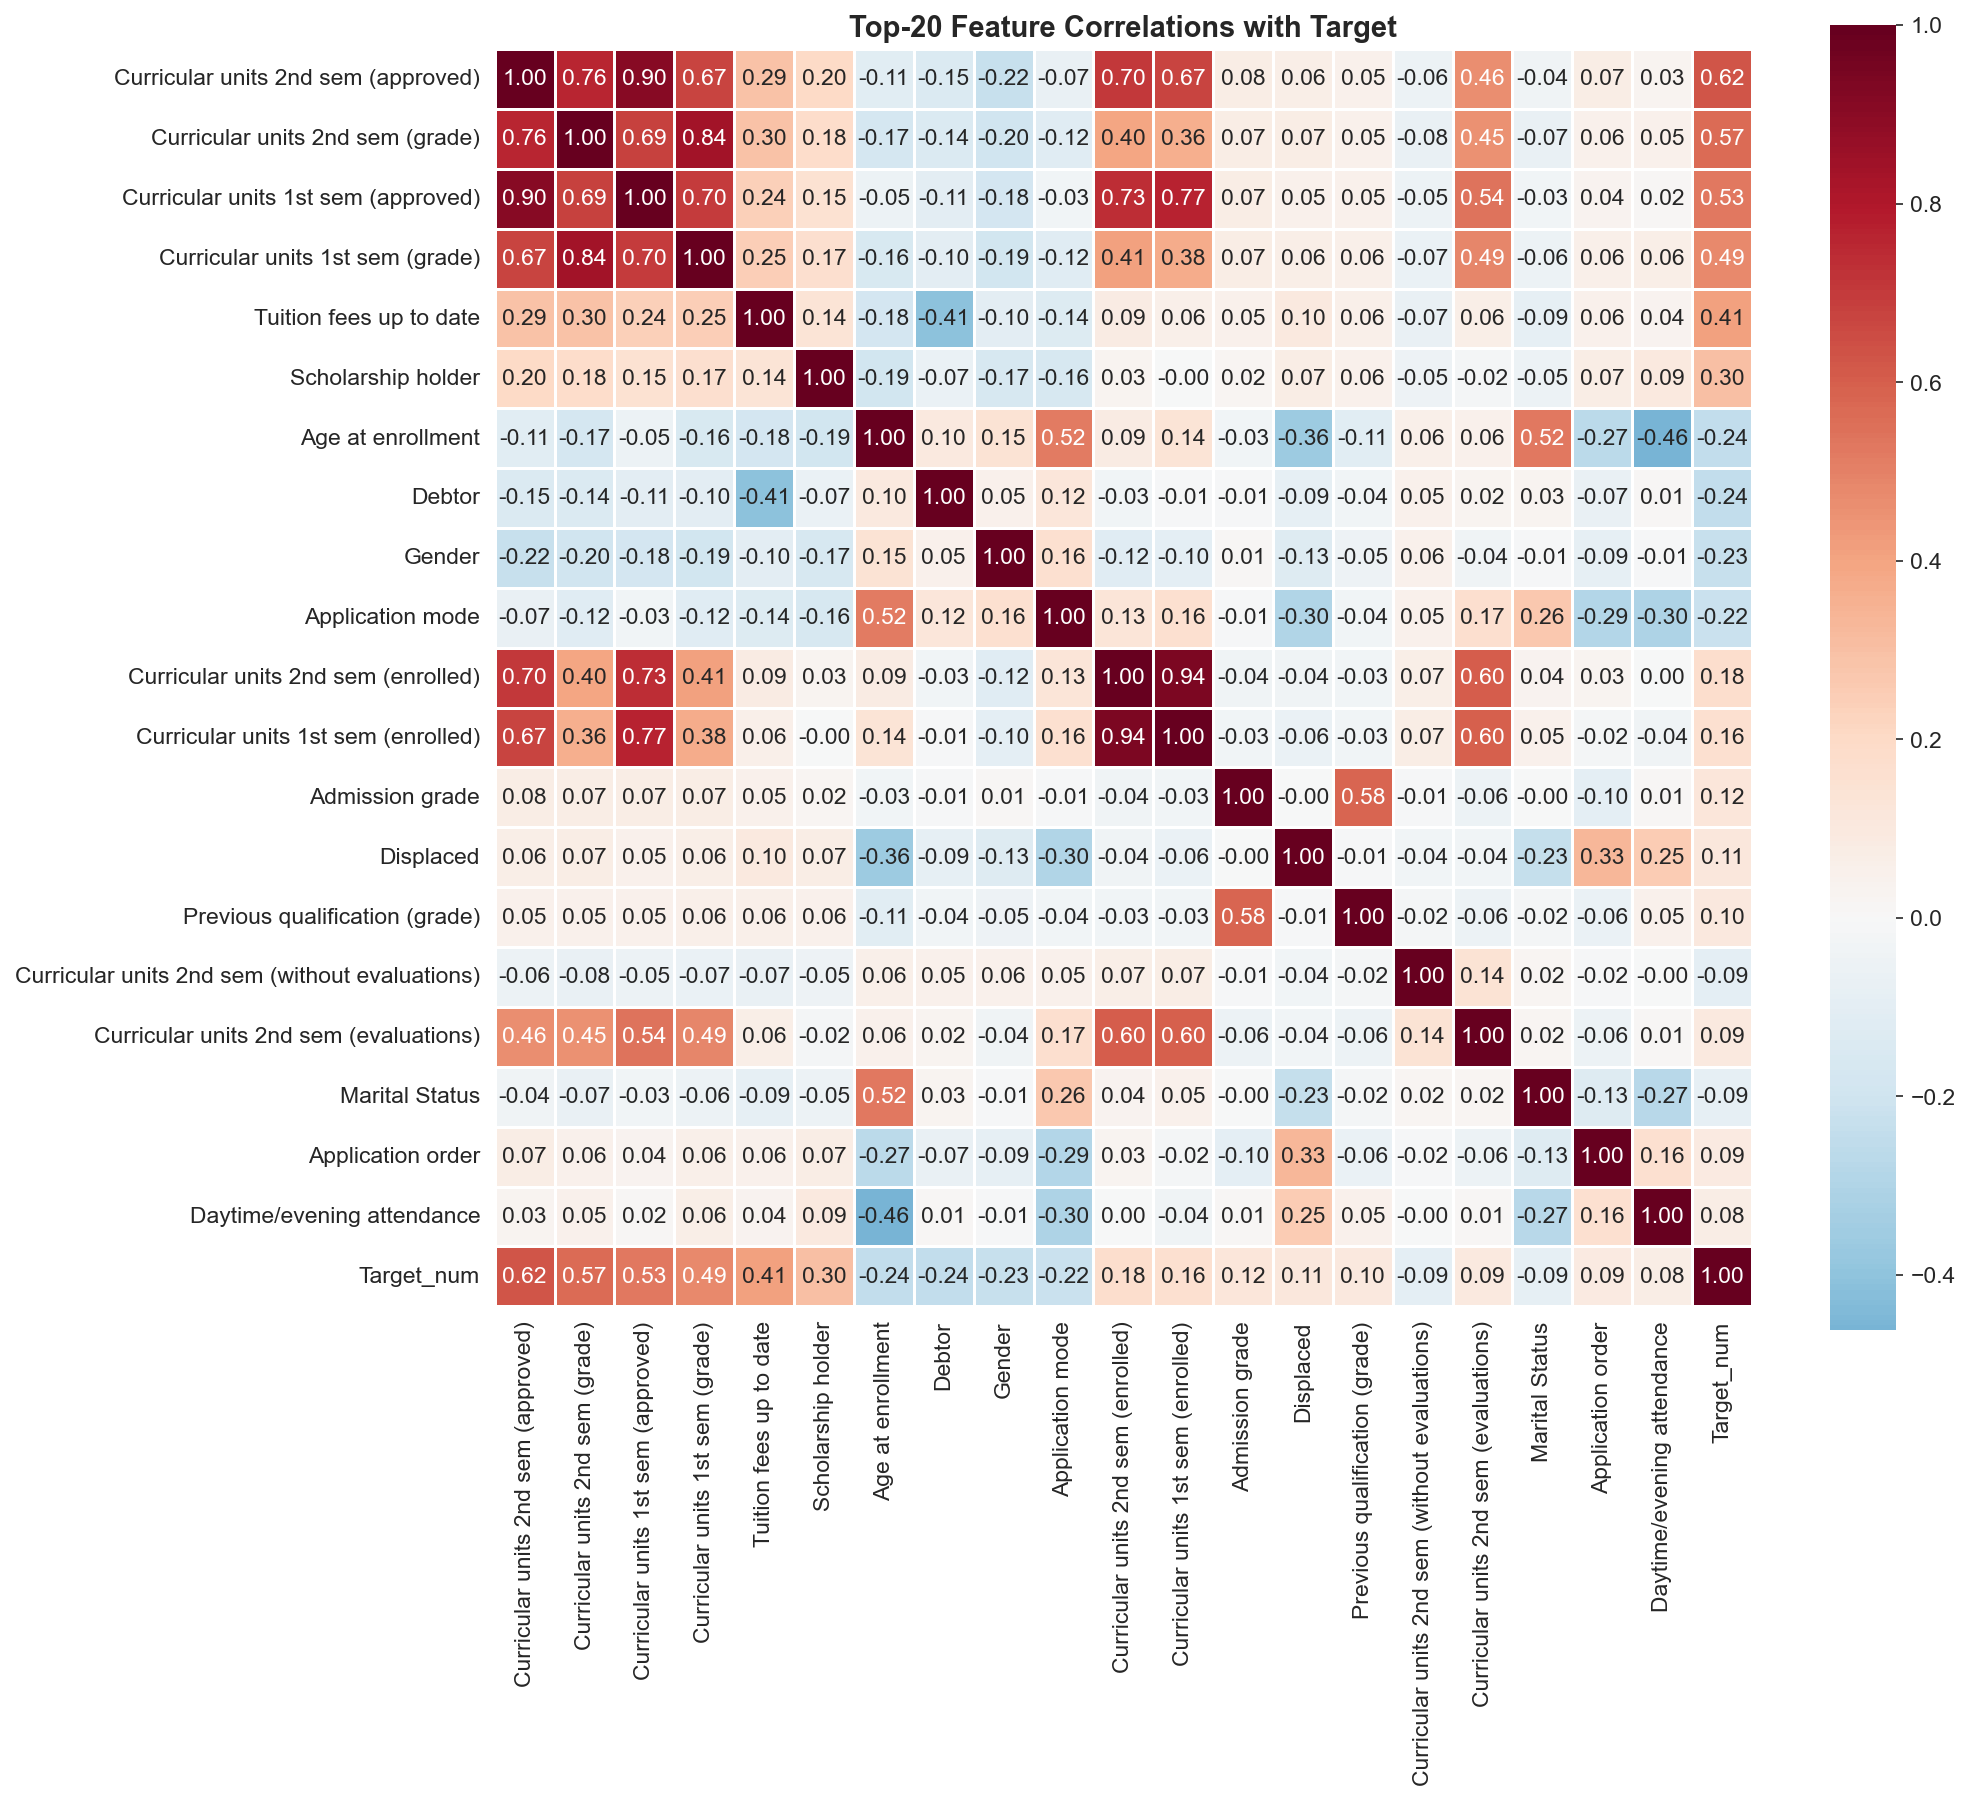
\includegraphics[width=\linewidth]{../data/plots/01_eda_correlation_heatmap.png}
\caption{Top-20 feature correlations with the target variable.}
\label{fig:eda_correlation}
\end{figure}

The data was split 70/15/15 into training (2,875), validation (664), and test (885) sets with stratified sampling to preserve class proportions.

\subsection{Data Visualization (t-SNE)}

We applied t-SNE with perplexity values of 5, 30, 50, and 100. The 2D projection at perplexity=30 (Figure~\ref{fig:tsne}) reveals that Graduate students form a relatively compact region, while Dropout students cluster separately. Enrolled students are scattered between both groups, consistent with their transitional academic status.

\begin{figure}[H]
\centering
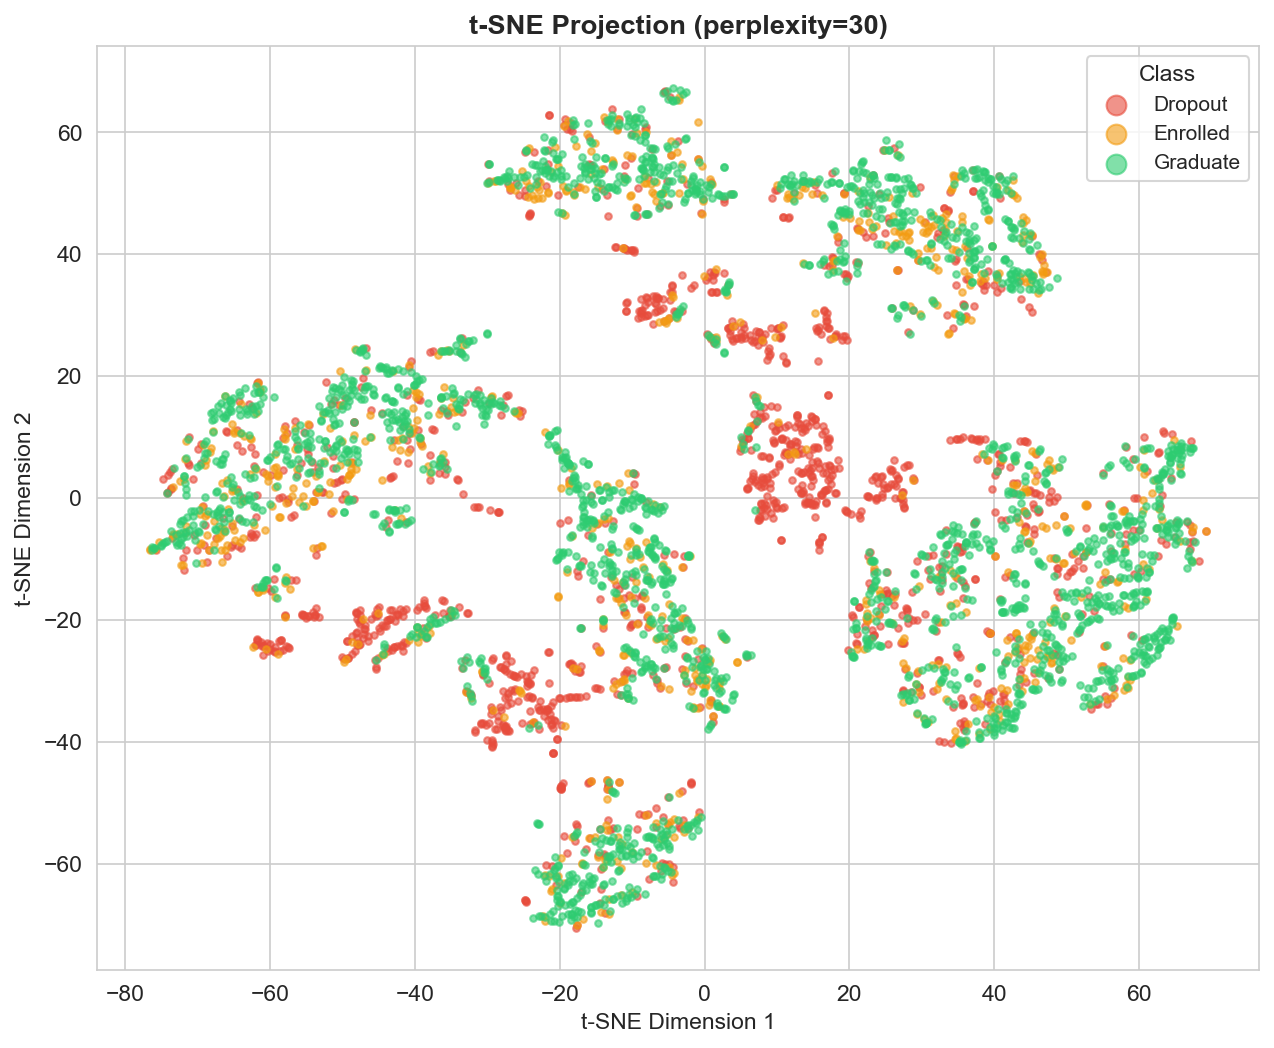
\includegraphics[width=\linewidth]{../data/plots/04_tsne_2d_best.png}
\caption{t-SNE 2D projection (perplexity=30) colored by class.}
\label{fig:tsne}
\end{figure}

The 3D projection (Figure~\ref{fig:tsne_3d}) provides additional spatial separation, further reducing overlap between Graduate and Dropout clusters, though the Enrolled class remains dispersed.

\begin{figure}[H]
\centering
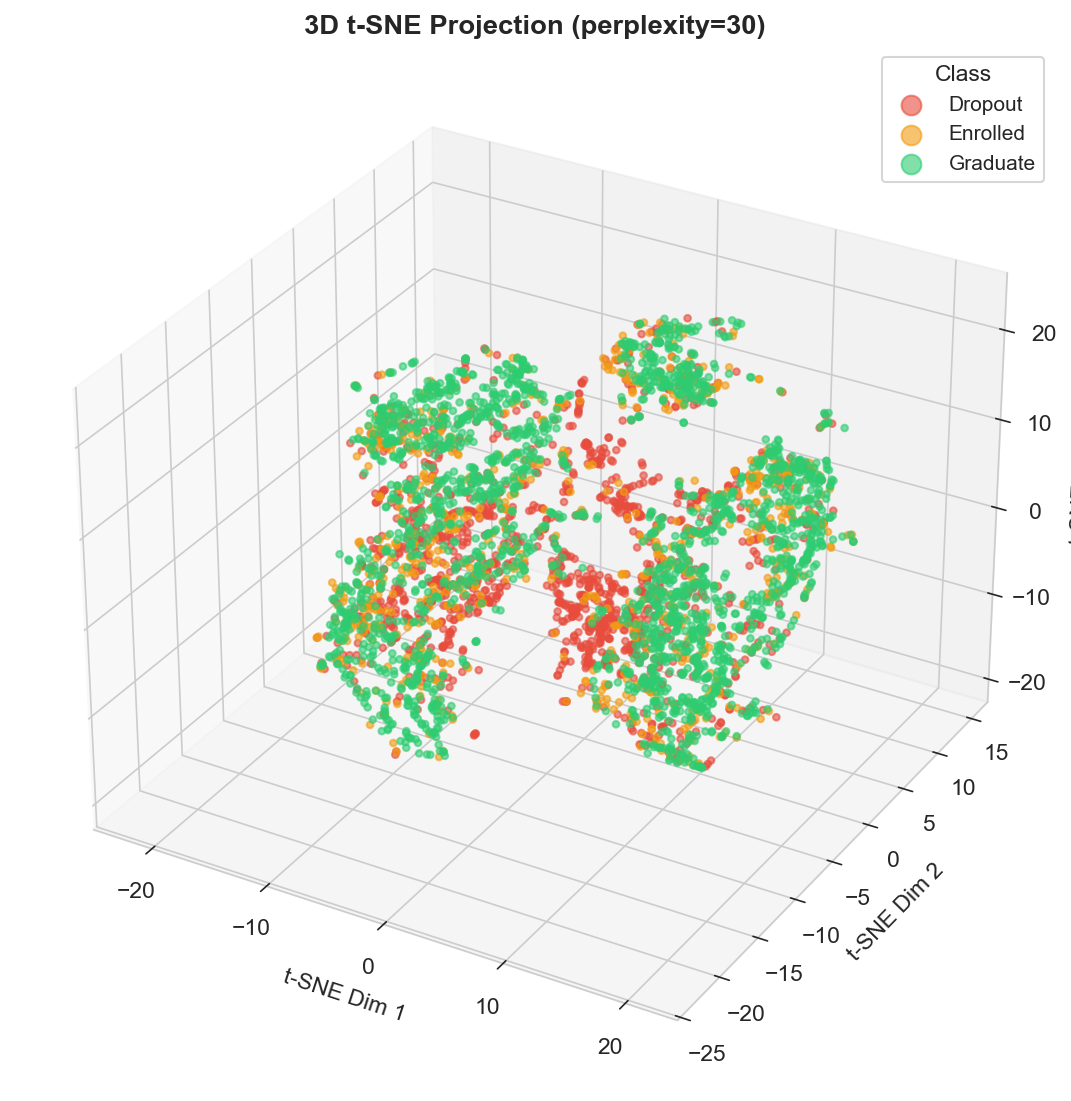
\includegraphics[width=\linewidth]{../data/plots/05_tsne_3d_best.png}
\caption{t-SNE 3D projection (perplexity=30) colored by class.}
\label{fig:tsne_3d}
\end{figure}

\subsection{Clustering Analysis}

Three algorithms were compared: K-Means, Agglomerative Hierarchical Clustering (ward, complete, average, single linkage), and DBSCAN.

K-Means with K=3 achieved the highest practical utility with ARI=0.177, producing clusters most aligned with true labels. DBSCAN, despite a higher normalized composite score driven by Silhouette on only 9 non-noise points, classified 99.8\% of data as noise (ARI=0.000), confirming it is unsuitable for this high-dimensional dataset. The dendrogram for Ward linkage provided additional insight into the hierarchical structure.

\begin{figure}[H]
\centering
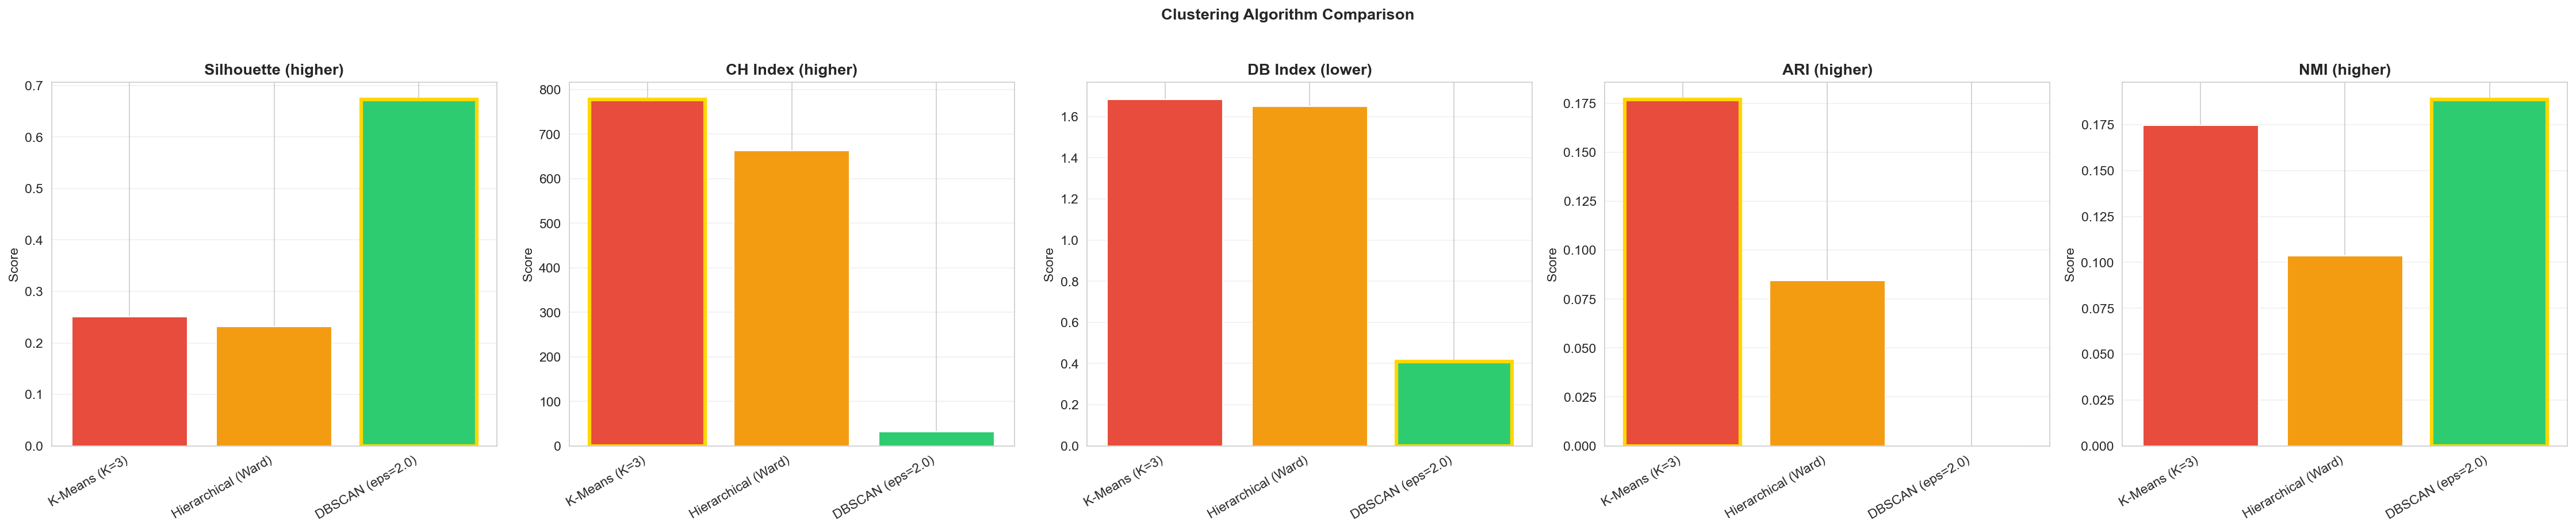
\includegraphics[width=\linewidth]{../data/plots/09_algorithm_comparison.png}
\caption{Clustering algorithm comparison across five metrics.}
\label{fig:clustering_comparison}
\end{figure}

\begin{figure}[H]
\centering
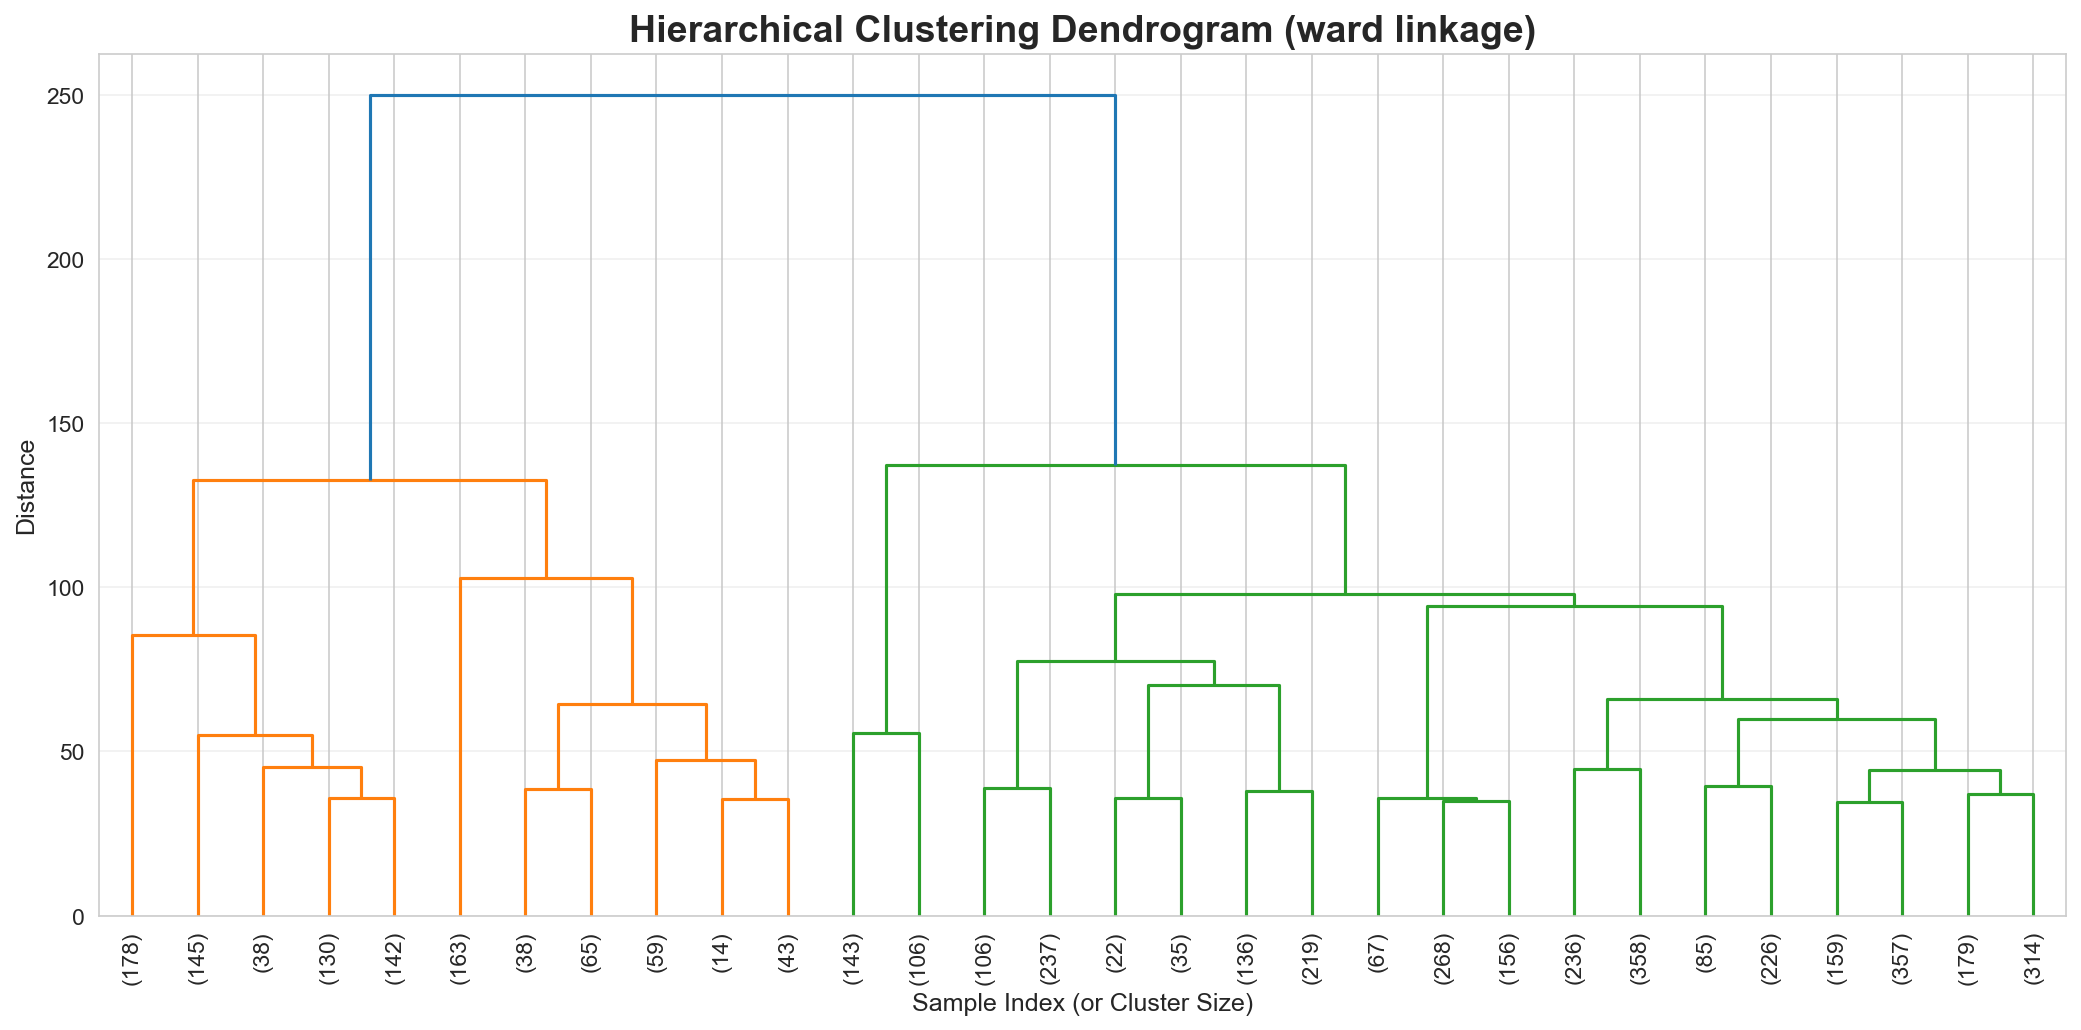
\includegraphics[width=\linewidth]{../data/plots/03_dendrogram_ward.png}
\caption{Hierarchical clustering dendrogram (Ward linkage).}
\label{fig:dendrogram}
\end{figure}

The dendrogram (Figure~\ref{fig:dendrogram}) shows that the data has a relatively flat hierarchical structure --- the three main clusters merge at similar distance levels, supporting K-Means' spherical cluster assumption. Among four linkage methods (ward/complete/average/single), Ward achieved the best ARI (0.084) with true labels.

A comparison of four linkage methods revealed that single and average linkages produced highly imbalanced clusters (one dominant cluster + outliers), while Ward and complete linkages generated more balanced partitions. This confirms that centroid-based methods (K-Means, Ward) are most appropriate for this dataset.

\subsection{Prediction: Training and Testing}

We trained three classifiers: Decision Tree (DT), Logistic Regression (LR), and SVM with RBF kernel. Models were evaluated on training, test, and entire sets.

Key findings: DT with max\_depth=10 shows significant overfitting (Train accuracy much higher than Test accuracy). LR provides stable generalization with minimal train-test gap. SVM achieves intermediate performance.

\begin{figure}[H]
\centering
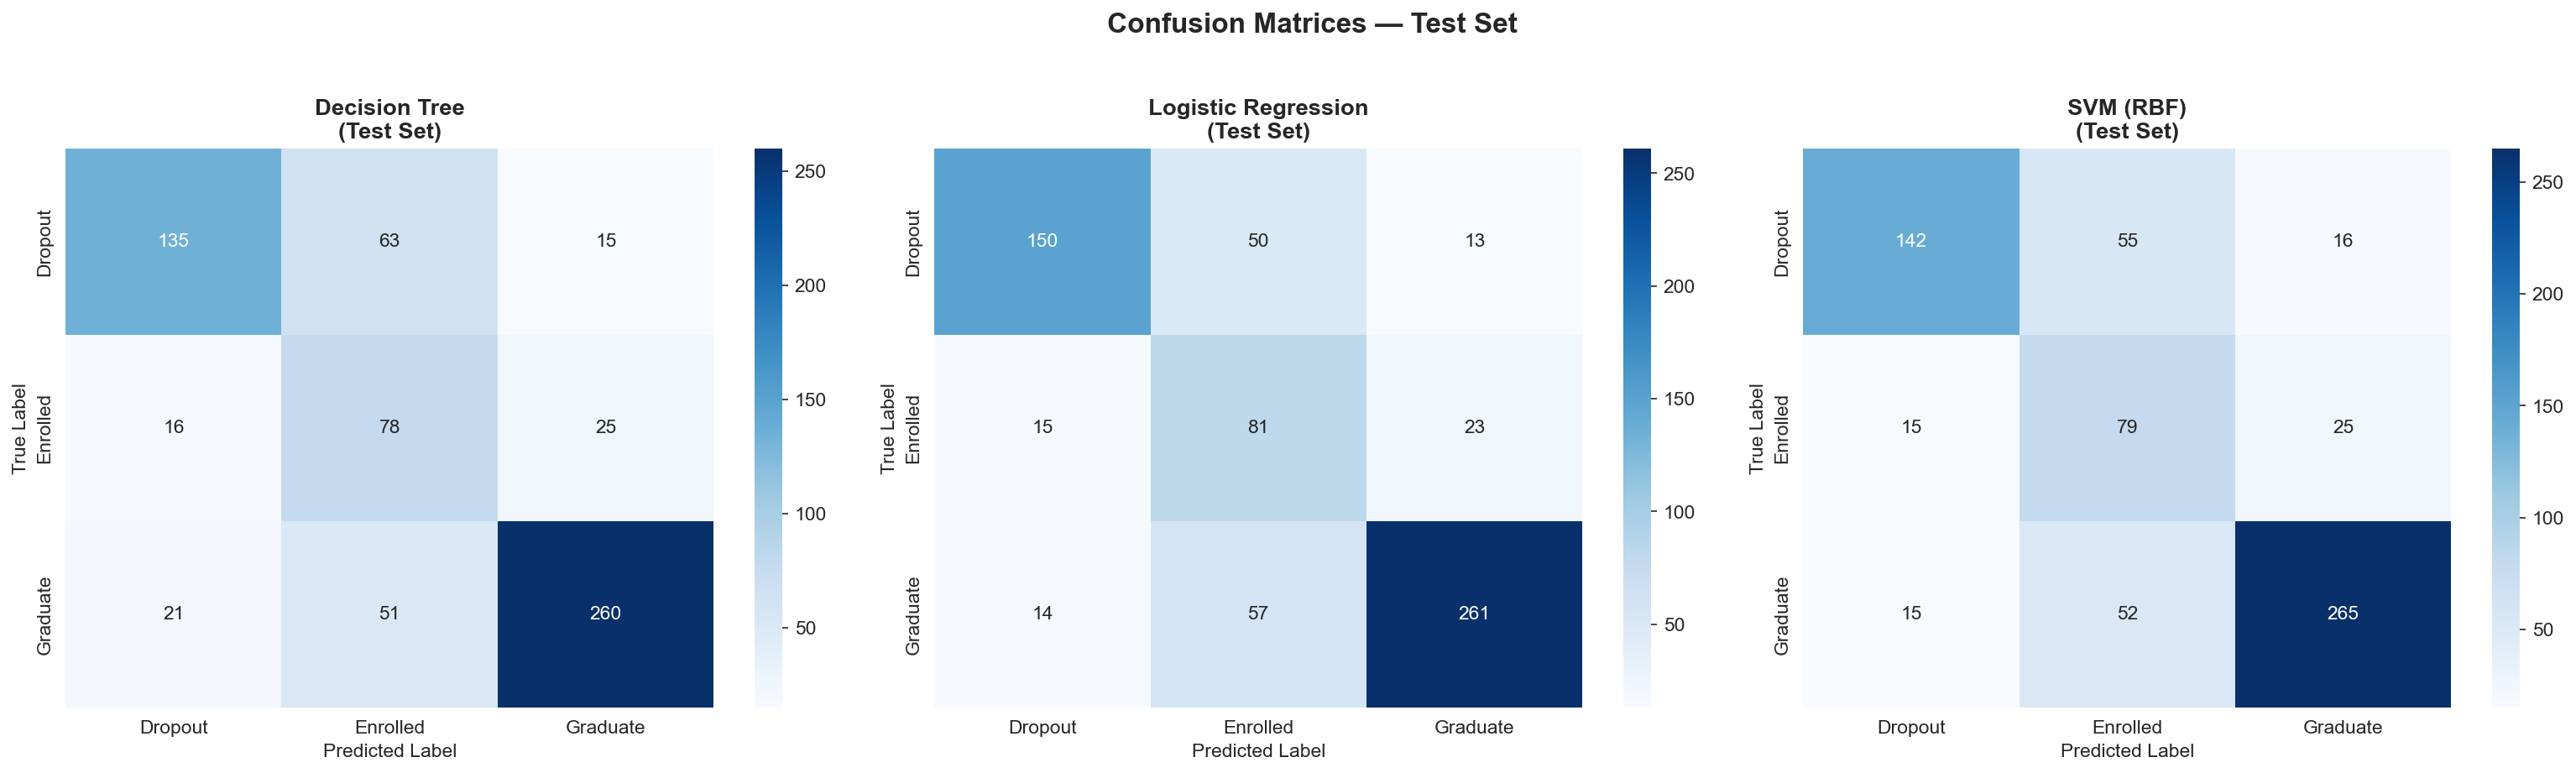
\includegraphics[width=\linewidth]{../data/plots/04_confusion_matrices_test.png}
\caption{Confusion matrices on the test set.}
\label{fig:cm_test}
\end{figure}

\begin{figure}[H]
\centering
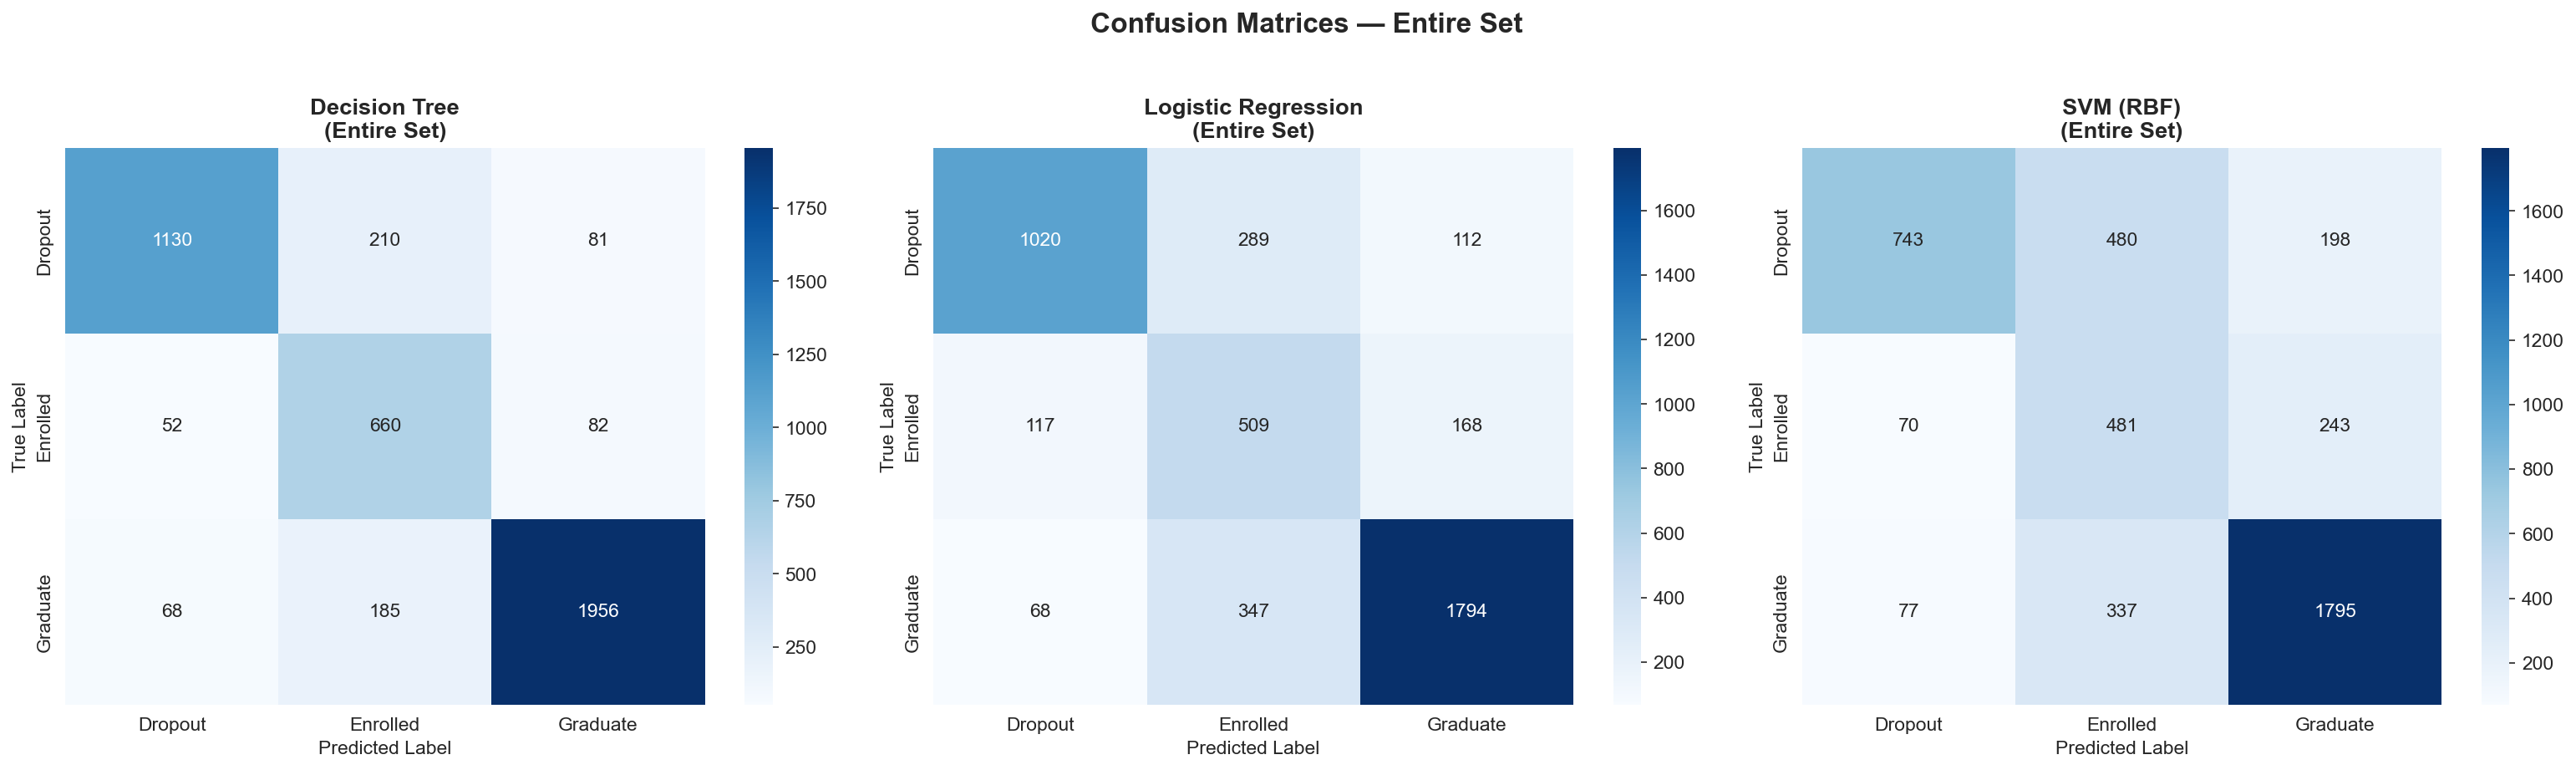
\includegraphics[width=\linewidth]{../data/plots/04_confusion_matrices_entire.png}
\caption{Confusion matrices on the entire dataset.}
\label{fig:cm_entire}
\end{figure}

The entire-set evaluation (Figure~\ref{fig:cm_entire}) reveals that DT's high accuracy on the entire set (84.1\%) is inflated by its memorization of training data, while LR (77.8\%) and SVM (74.2\%) show more consistent performance. The gap between train and test accuracy serves as a reliable overfitting indicator: DT (91.0\% vs 71.1\%), LR (78.2\% vs 76.8\%), SVM (74.1\% vs 75.3\%).

\begin{figure}[H]
\centering
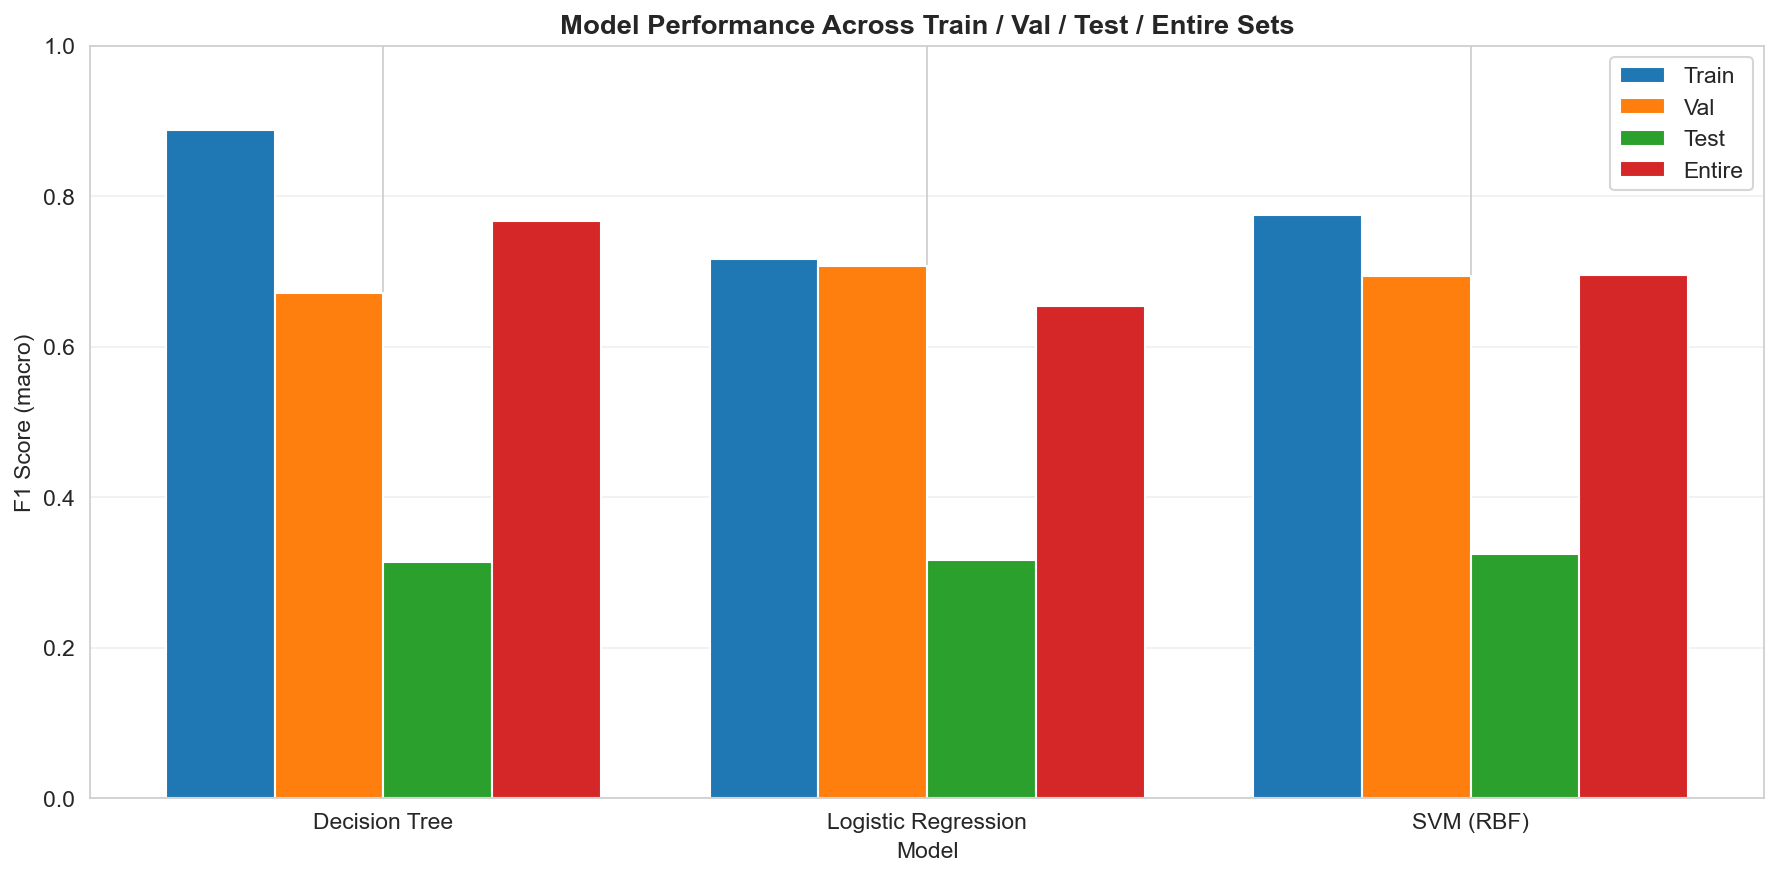
\includegraphics[width=\linewidth]{../data/plots/04_model_comparison_three_sets.png}
\caption{Model performance across train, validation, test, and entire sets.}
\label{fig:three_set_comparison}
\end{figure}

The per-class analysis shows that all models achieve highest recall for Graduate ($\sim$85--91\%) and lowest for Enrolled ($\sim$30--50\%). This is consistent with the class imbalance (Graduate: 49.9\%, Enrolled: 18.0\%) and the transitional nature of enrolled students.

\subsection{Evaluation and Model Choice}

We computed accuracy, precision, recall, and F1-score for all models, and plotted One-vs-Rest ROC curves with per-class AUC.

\textbf{Improvement via validation:} Validation curves guided hyperparameter selection. GridSearchCV was applied to each model:
\begin{itemize}
\item DT: tuned max\_depth, min\_samples\_split, min\_samples\_leaf
\item LR: tuned C and solver
\item SVM: tuned C and gamma
\end{itemize}

\begin{figure}[H]
\centering
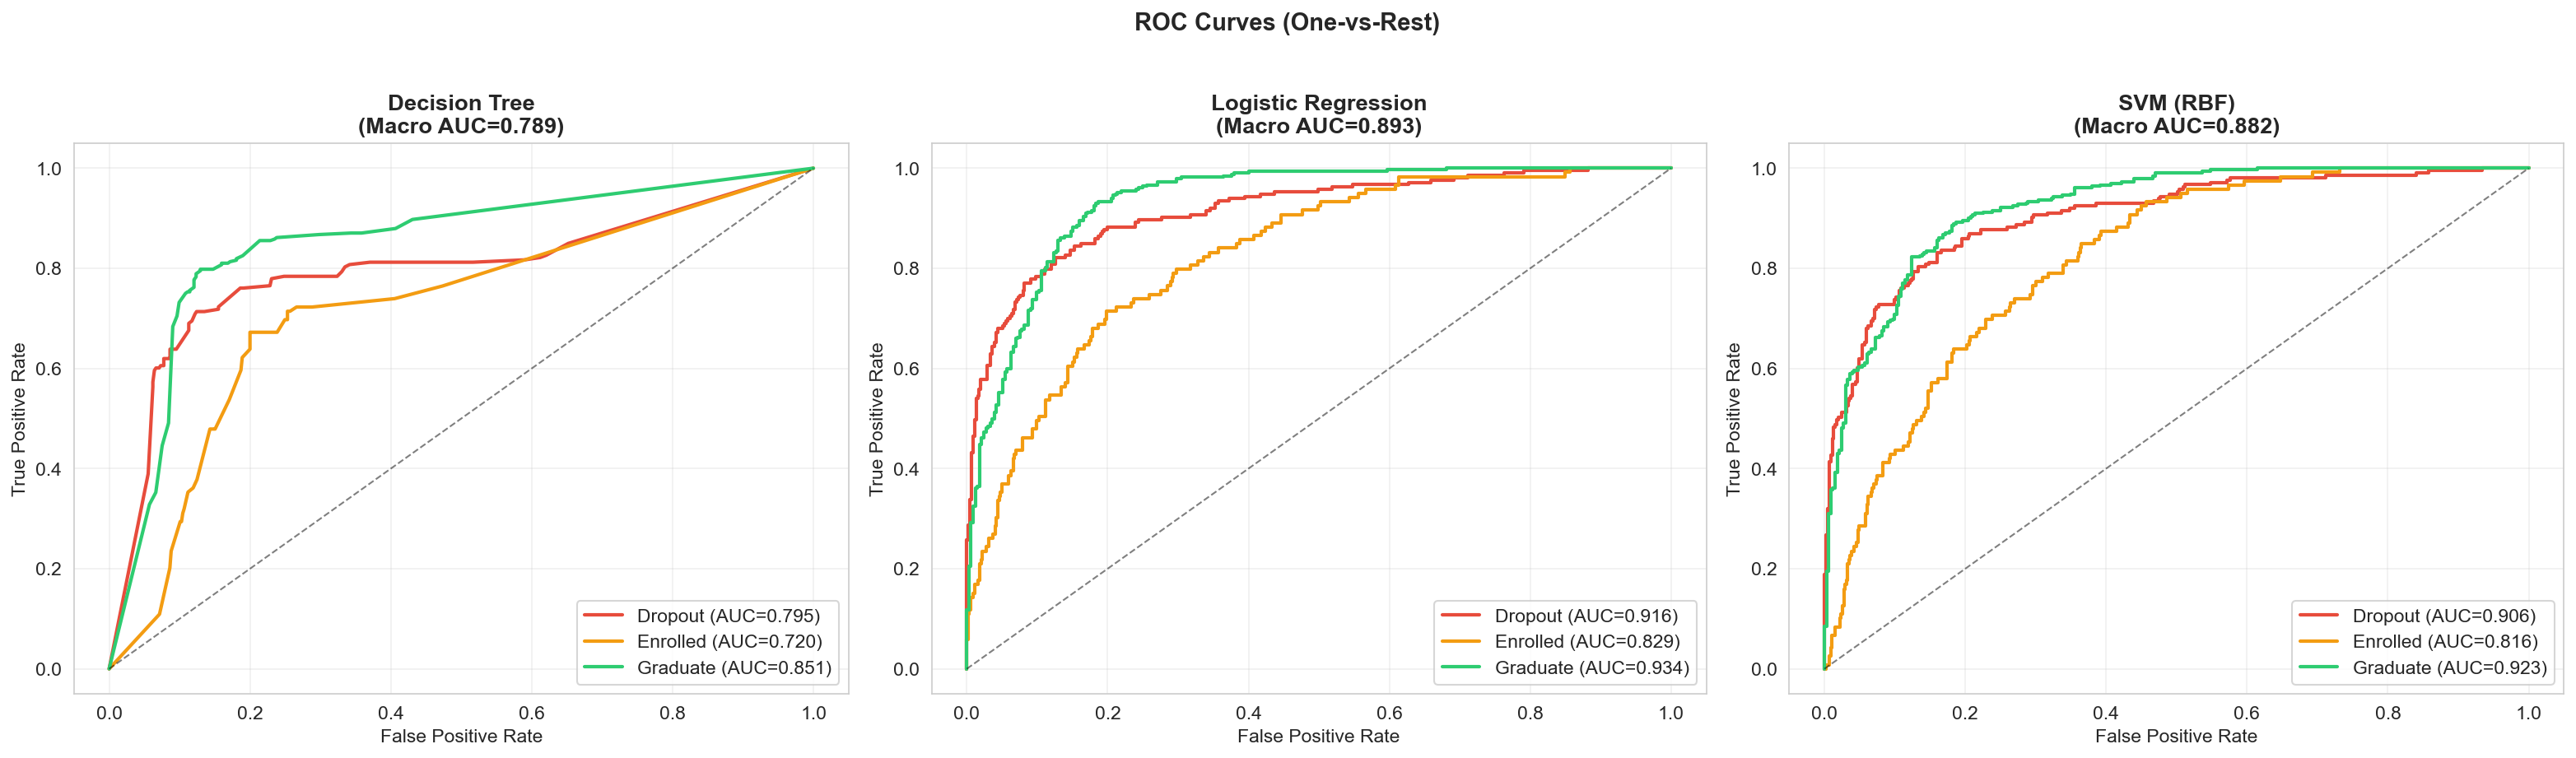
\includegraphics[width=\linewidth]{../data/plots/05_roc_curves.png}
\caption{ROC curves (One-vs-Rest) for all baseline models.}
\label{fig:roc}
\end{figure}

\textbf{Validation curve analysis} (Figure~\ref{fig:valcurve}) reveals model-specific sensitivity to hyperparameters:

\begin{figure}[H]
\centering
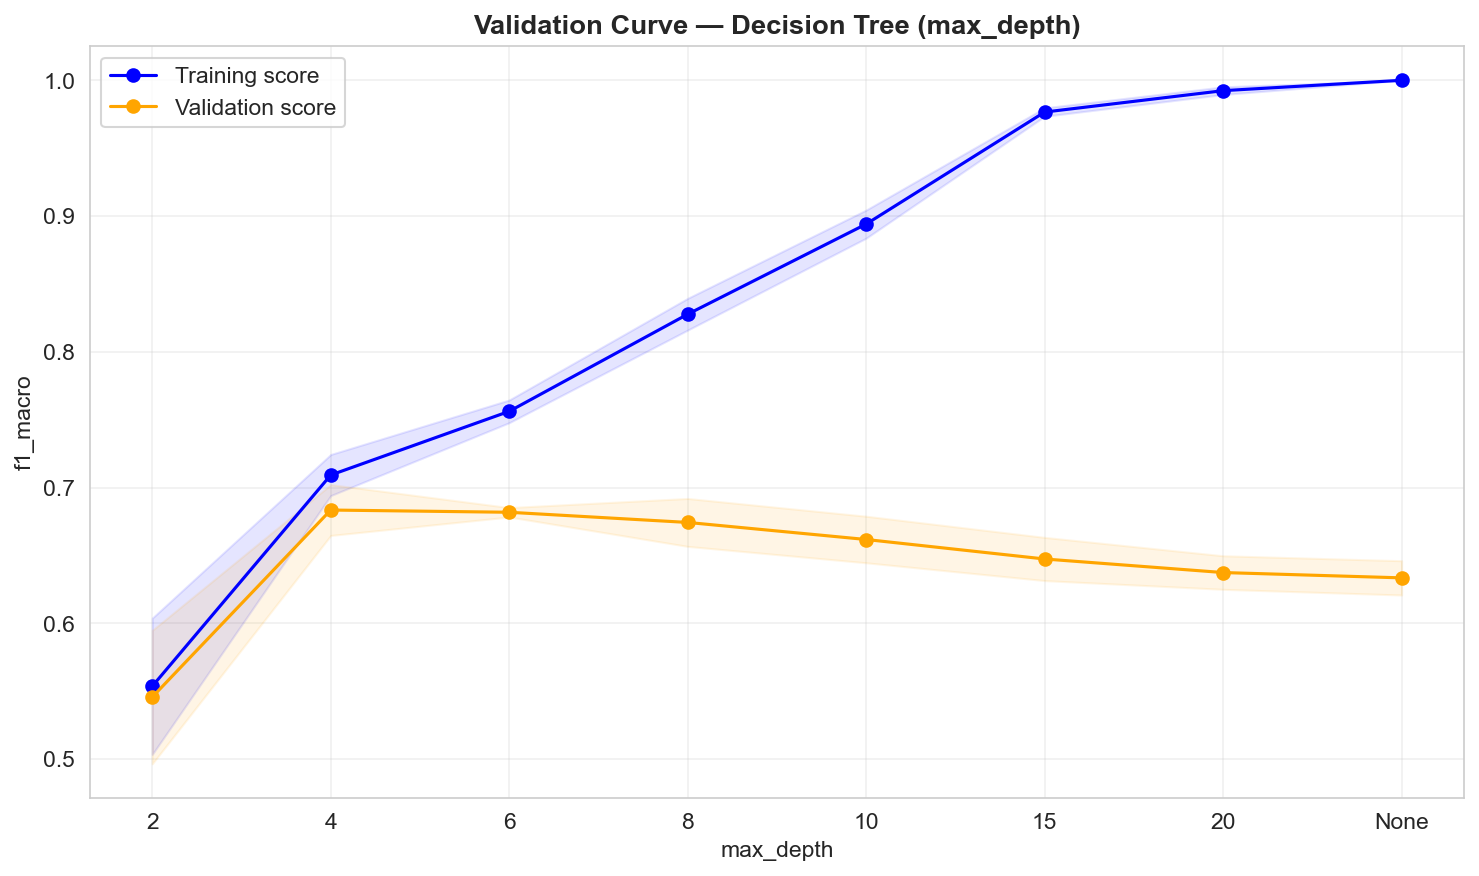
\includegraphics[width=0.49\linewidth]{../data/plots/05_valcurve_dt_depth.png}
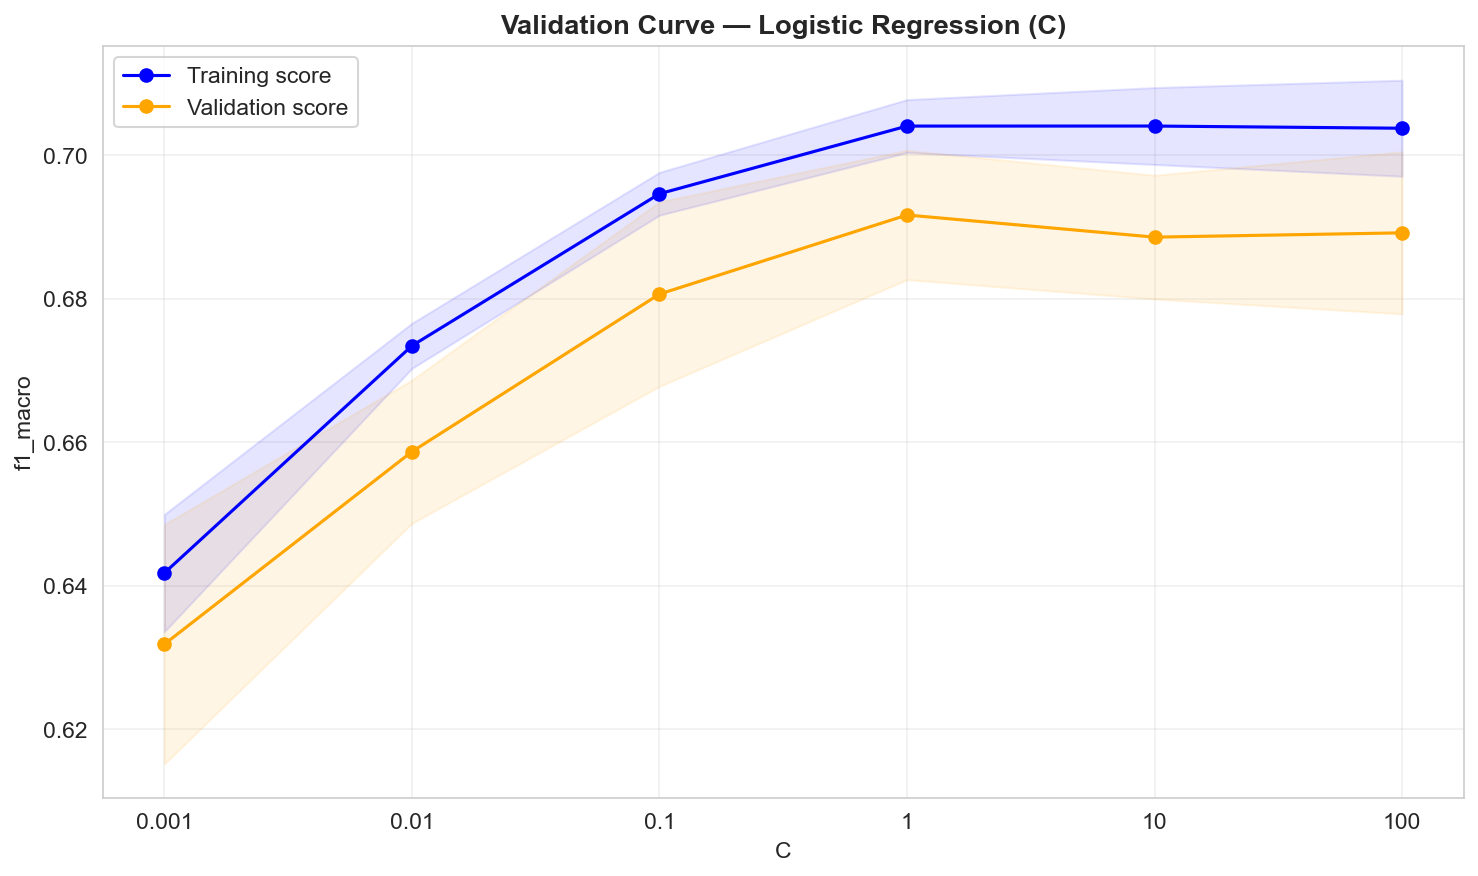
\includegraphics[width=0.49\linewidth]{../data/plots/05_valcurve_lr_c.png}
\caption{Validation curves for Decision Tree (left) and Logistic Regression (right).}
\label{fig:valcurve}
\end{figure}

\begin{itemize}
\item \textbf{DT (max\_depth):} Clear overfitting beyond depth 8 --- training score continues rising while validation score declines. Optimal range: 5--7.
\item \textbf{LR (C):} Relatively insensitive to C, suggesting the linear assumption is the primary bottleneck, not regularization strength.
\item \textbf{SVM (C, gamma):} Both parameters significantly affect performance. High gamma causes severe overfitting.
\end{itemize}

\textbf{Learning curves} (Figure~\ref{fig:learning_curves}) show that all models benefit from more data, with LR and SVM showing the steepest improvement in the early stages.

\begin{figure}[H]
\centering
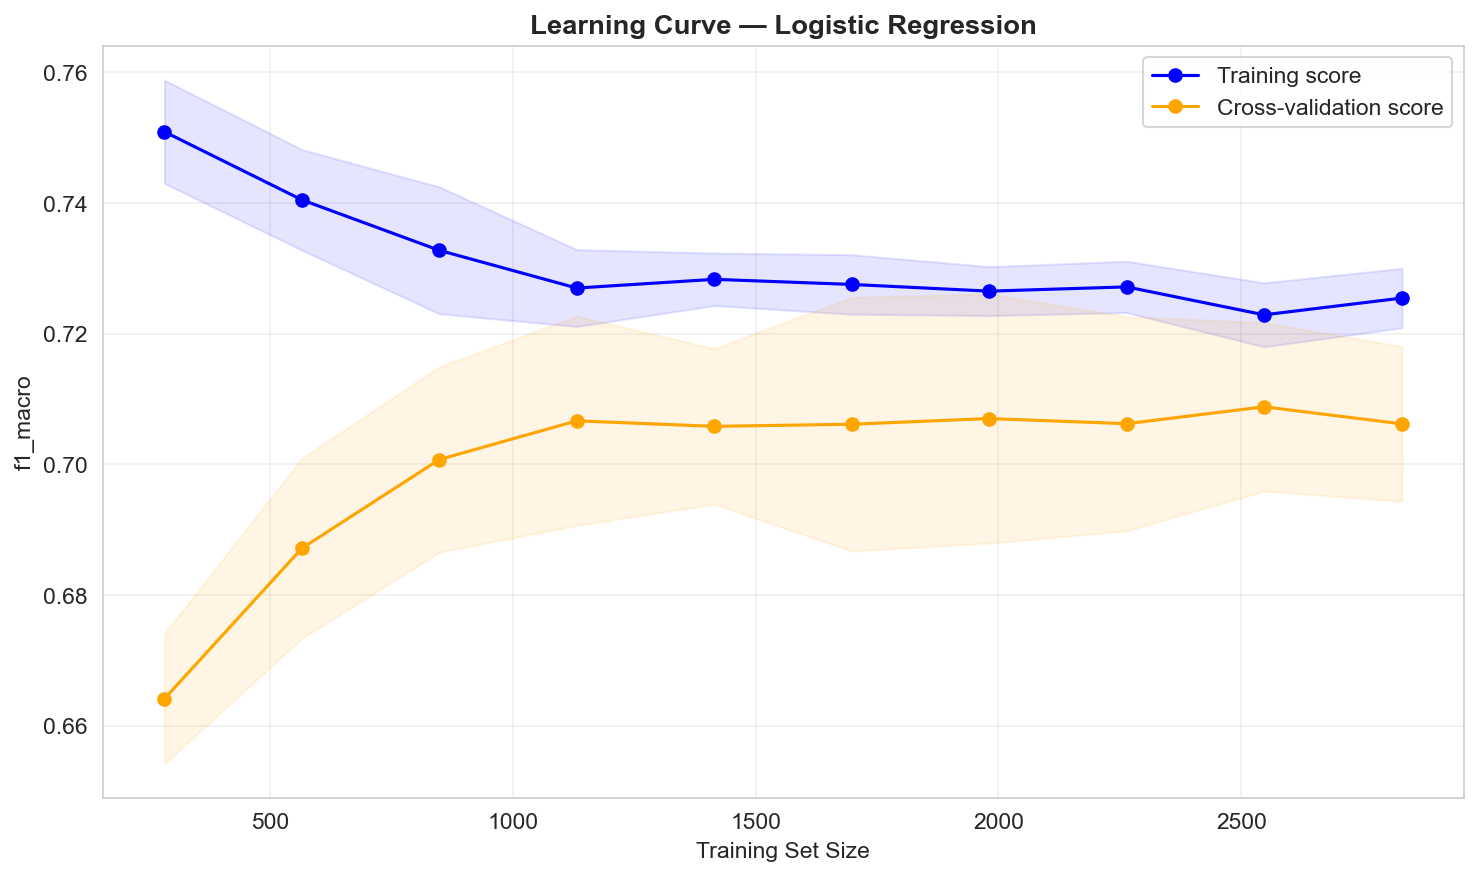
\includegraphics[width=\linewidth]{../data/plots/05_learning_curve_lr.png}
\caption{Learning curve for Logistic Regression.}
\label{fig:learning_curves}
\end{figure}

\textbf{Tuning results:} GridSearchCV produced measurable improvements (Table~\ref{tab:tuning}).

\begin{table}[H]
\centering
\caption{Baseline vs.\ tuned model performance on test set.}
\label{tab:tuning}
\begin{tabular}{lccc}
\toprule
Model & Baseline F1 & Tuned F1 & Improvement \\
\midrule
Decision Tree & 0.6211 & 0.6861 & +0.0650 \\
Logistic Regression & 0.6996 & 0.7061 & +0.0065 \\
SVM (RBF) & 0.6677 & 0.6639 & $-$0.0038 \\
\bottomrule
\end{tabular}
\end{table}

\begin{figure}[H]
\centering
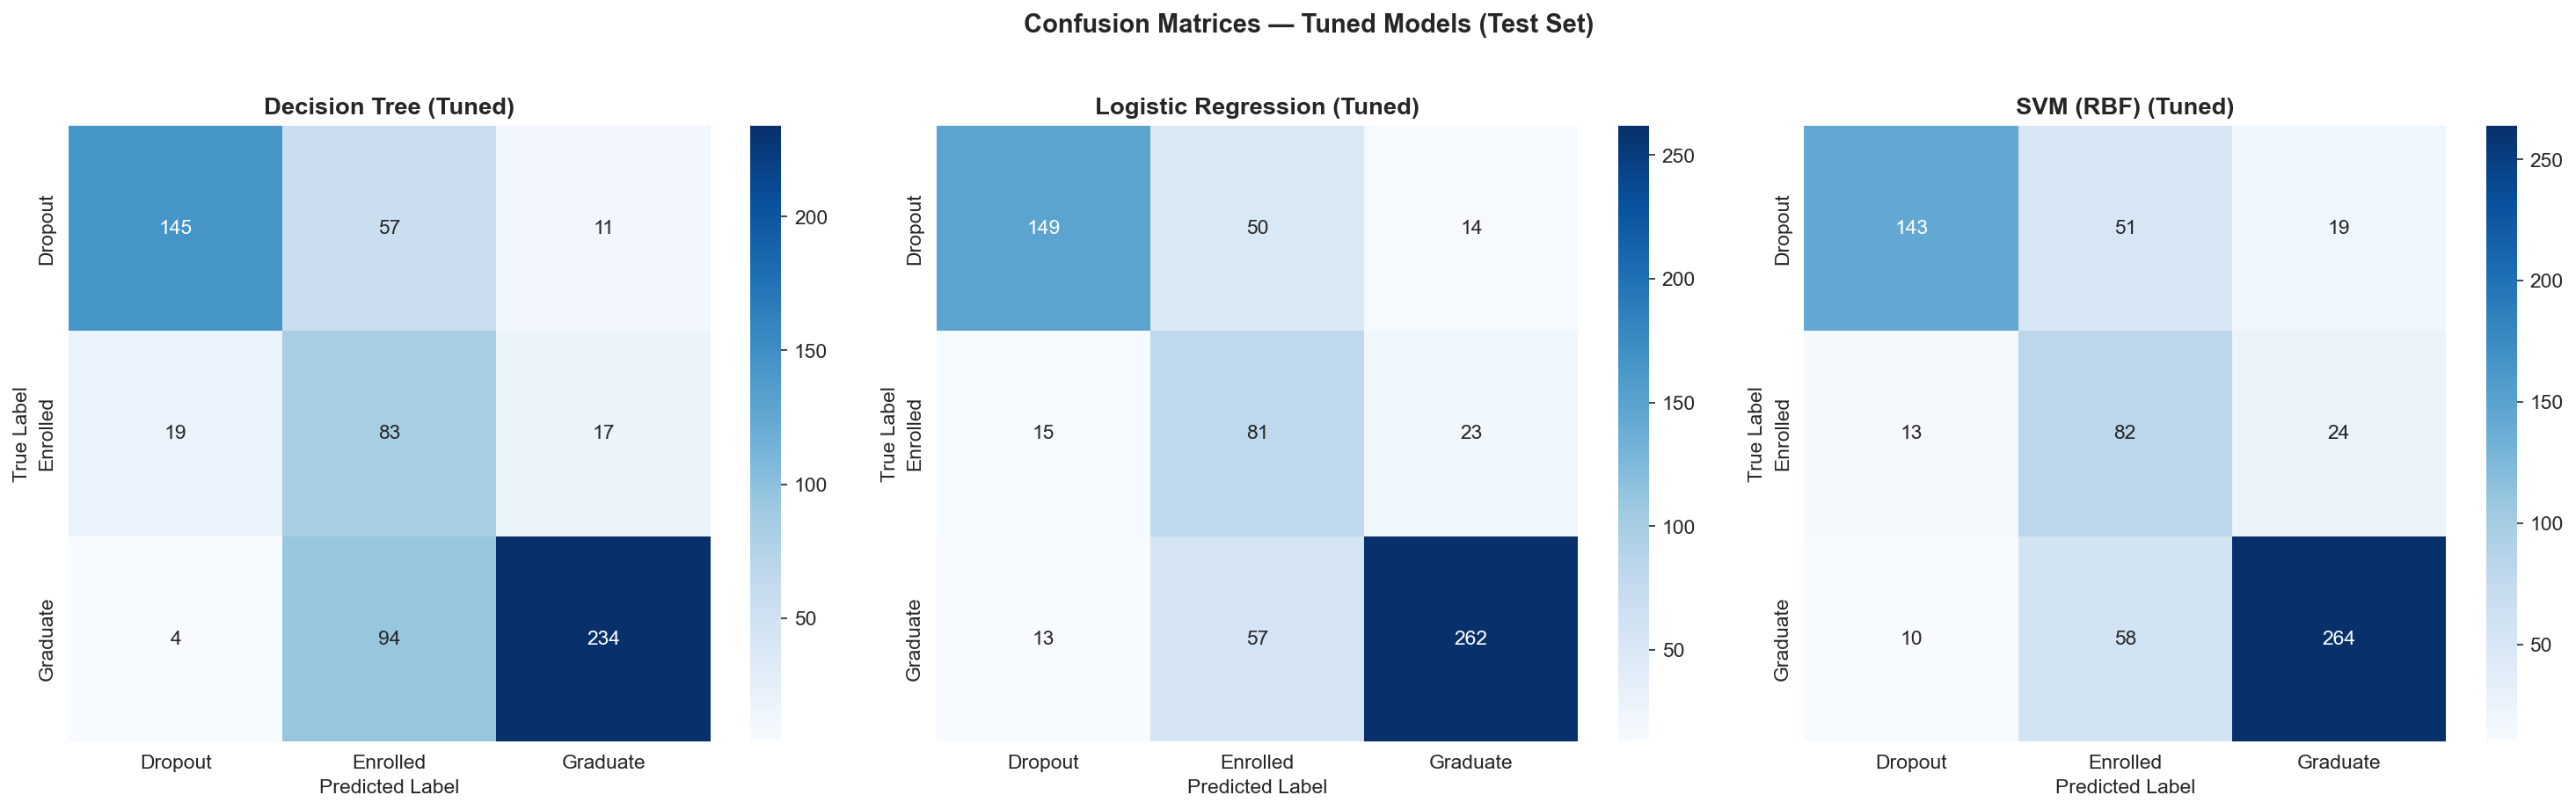
\includegraphics[width=\linewidth]{../data/plots/05_confusion_matrices_tuned.png}
\caption{Confusion matrices for tuned models on the test set.}
\label{fig:cm_tuned}
\end{figure}

The tuned models showed measurable improvement, particularly for Decision Tree where reduced max\_depth significantly decreased overfitting. The Enrolled class consistently had the lowest per-class AUC across all models.

% ====================
\section{Open-ended Exploration}

\subsection{Ensemble Methods}

We introduced Random Forest and Gradient Boosting classifiers. After GridSearchCV tuning, both ensemble methods outperformed the individual baseline models.

\subsection{Cross-Validation Comparison}

A unified 5-fold cross-validation comparison across all five model classes revealed the relative strengths of each approach, with ensemble methods achieving higher and more stable F1-scores.

\subsection{Feature Importance Analysis}

Feature importance scores from the best tree-based ensemble (Figure~\ref{fig:feature_importance}) confirm that academic performance metrics---approval rates and grade scores from both semesters---are the dominant predictive signals. Performance plateaus around 30--40 features, confirming that the top academic performance metrics are sufficient for strong classification.

\begin{figure}[H]
\centering
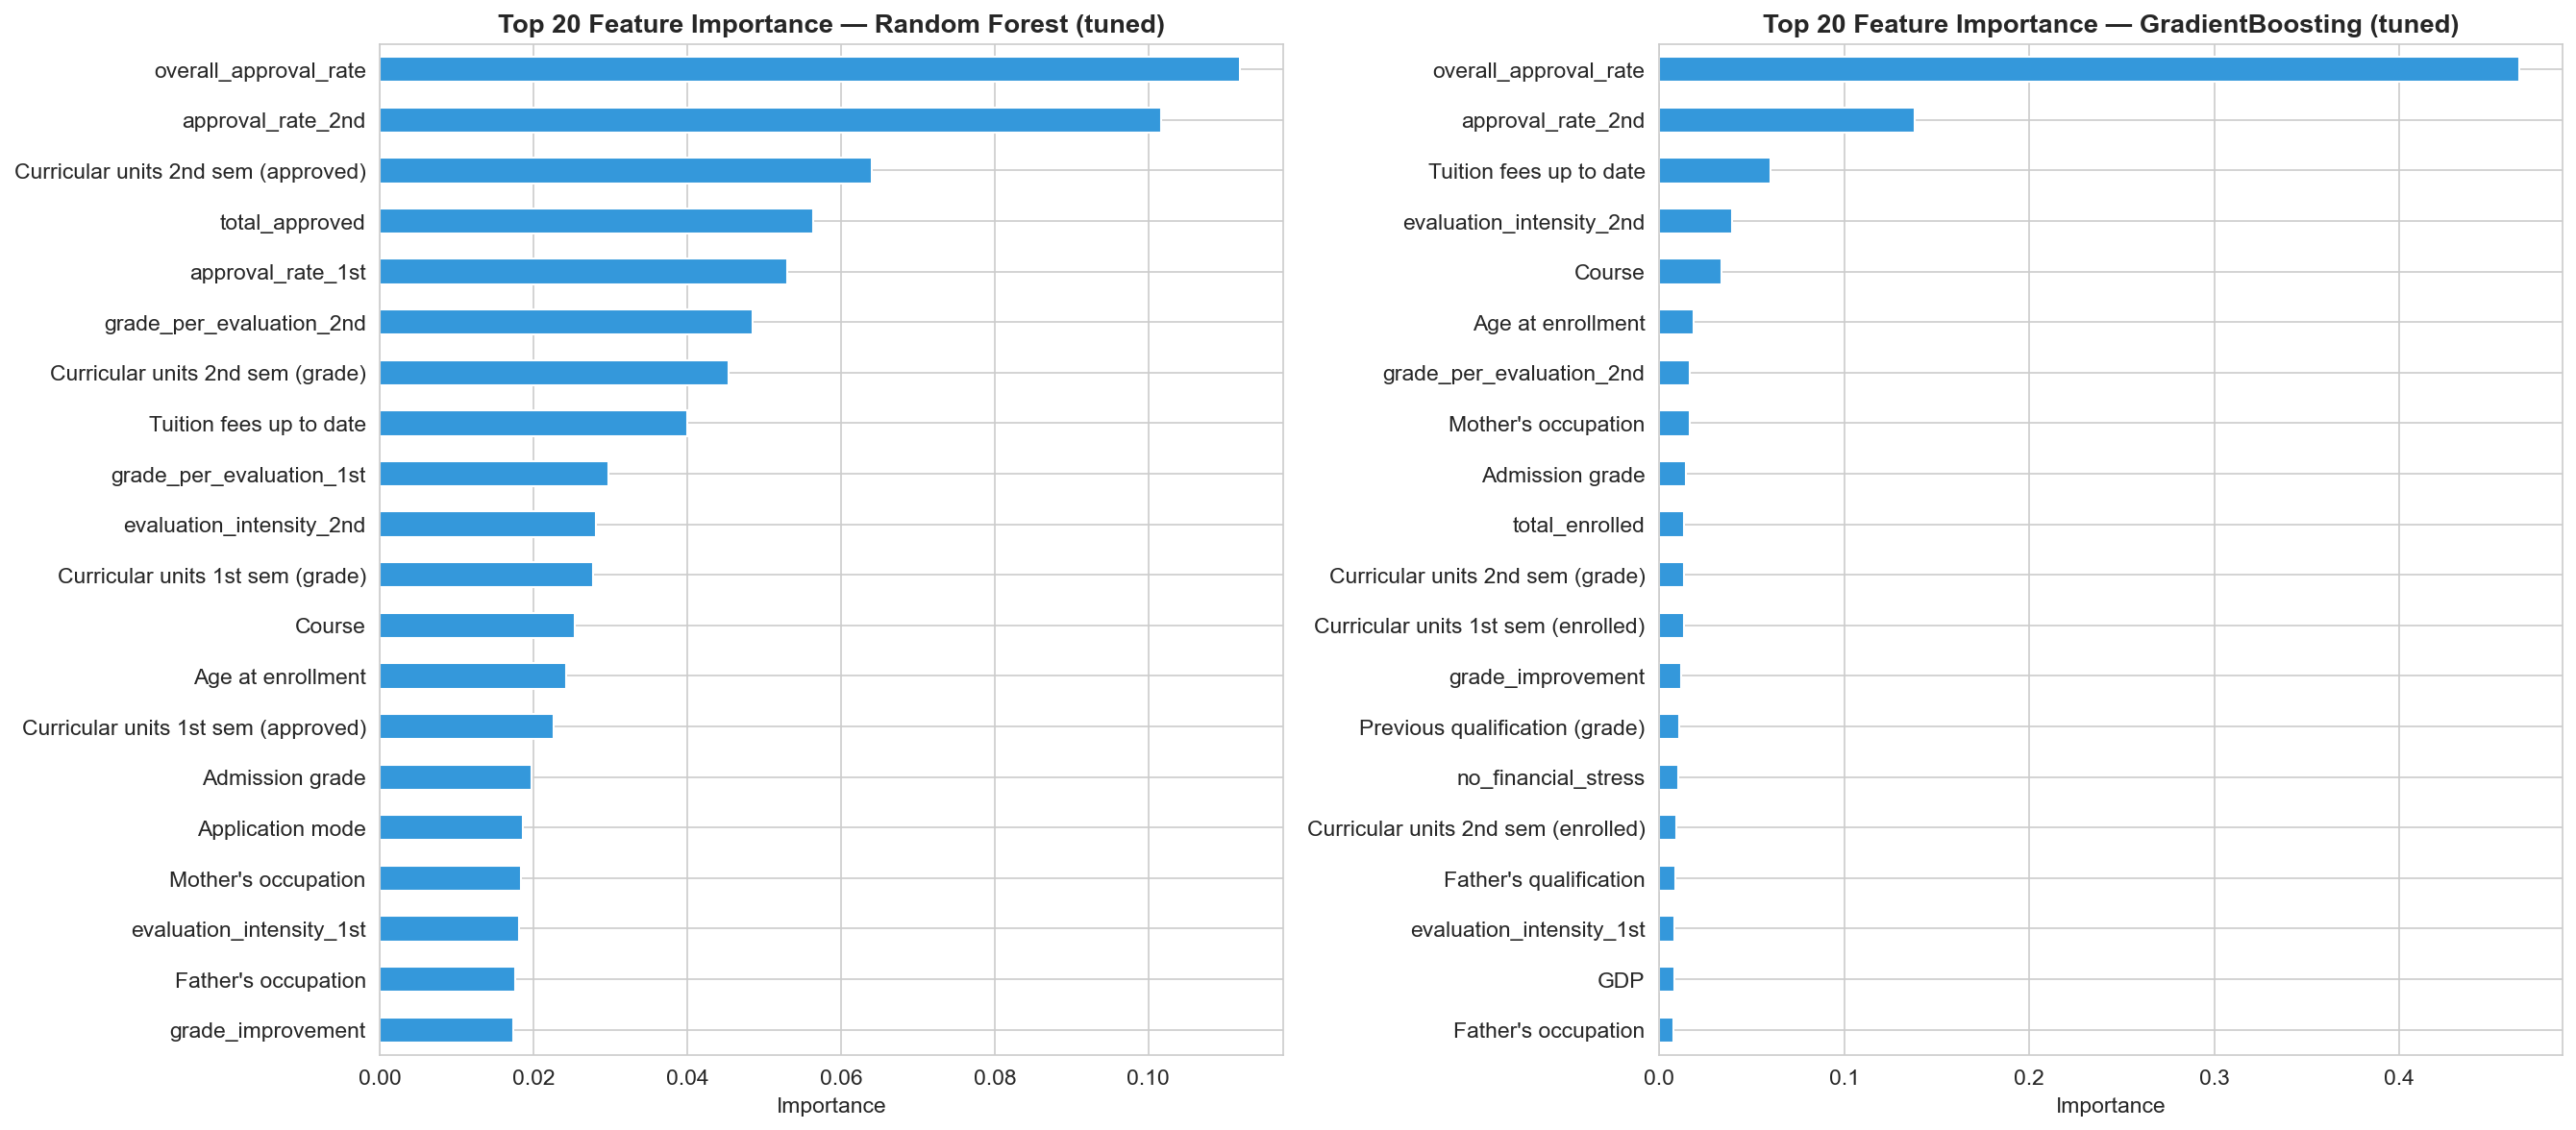
\includegraphics[width=\linewidth]{../data/plots/06_feature_importance.png}
\caption{Top feature importances from the ensemble model.}
\label{fig:feature_importance}
\end{figure}

A unified 5-fold cross-validation across all five model classes (Figure~\ref{fig:cv_boxplot}) confirms that ensemble methods achieve higher and more stable F1-scores than individual classifiers.

\begin{figure}[H]
\centering
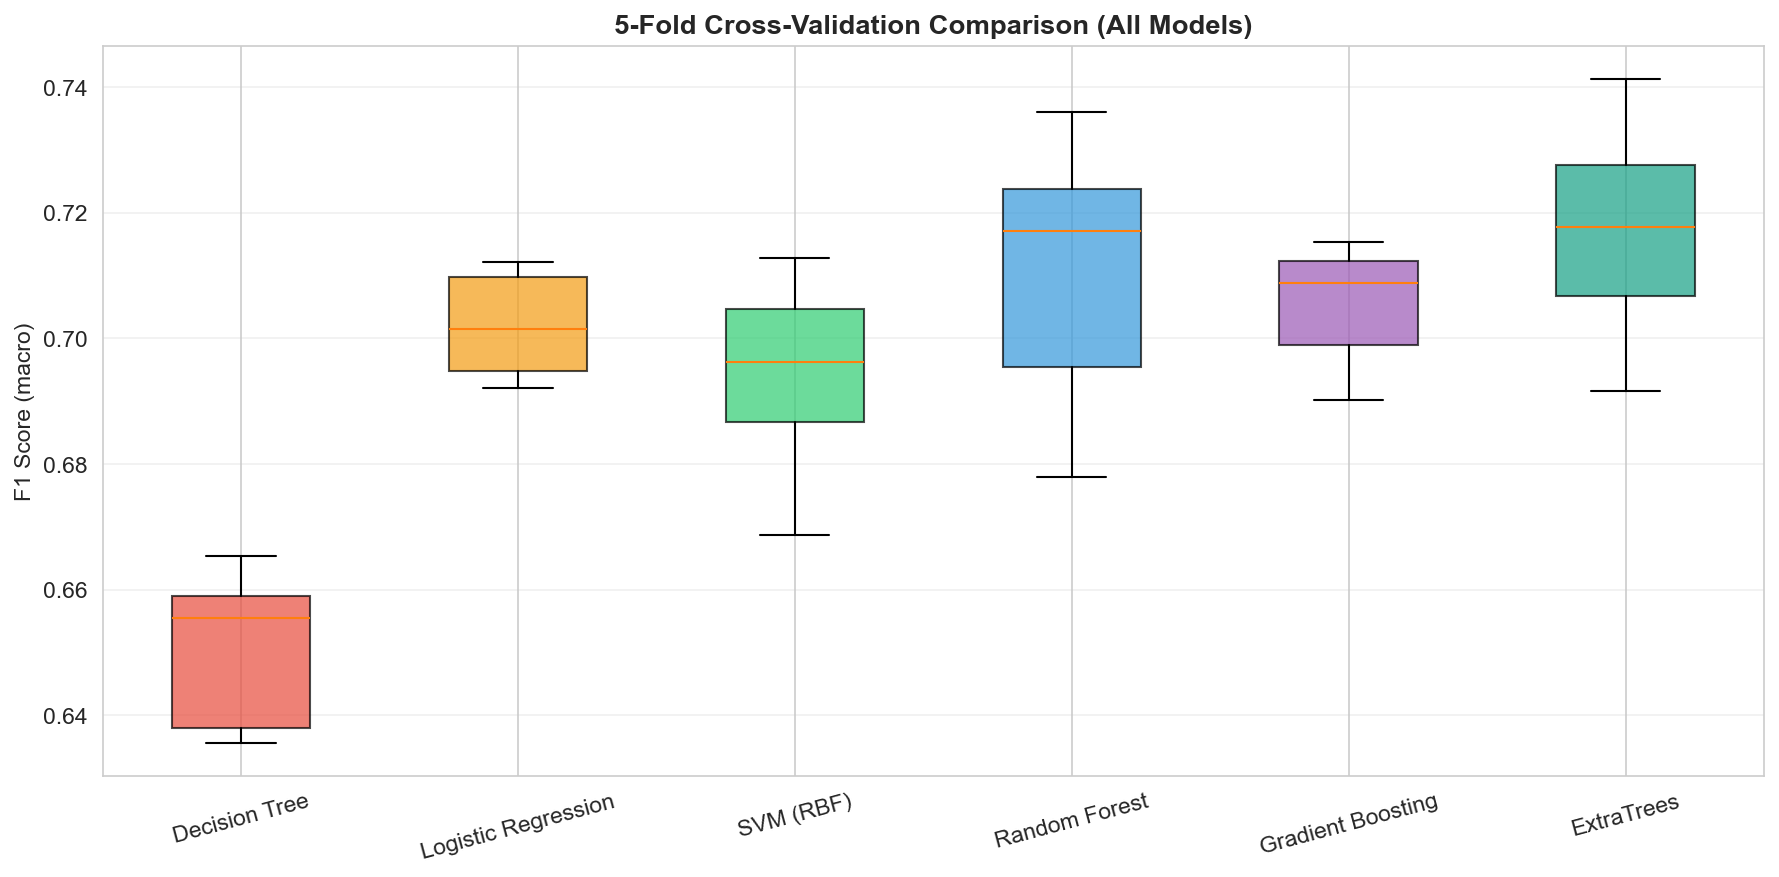
\includegraphics[width=\linewidth]{../data/plots/06_cv_comparison_all_models.png}
\caption{5-fold CV F1 (macro) comparison across all models.}
\label{fig:cv_boxplot}
\end{figure}

Evaluating model performance with Top-K features (Figure~\ref{fig:feature_selection}) shows performance plateauing around 30--40 features, confirming that academic performance metrics dominate prediction.

\begin{figure}[H]
\centering
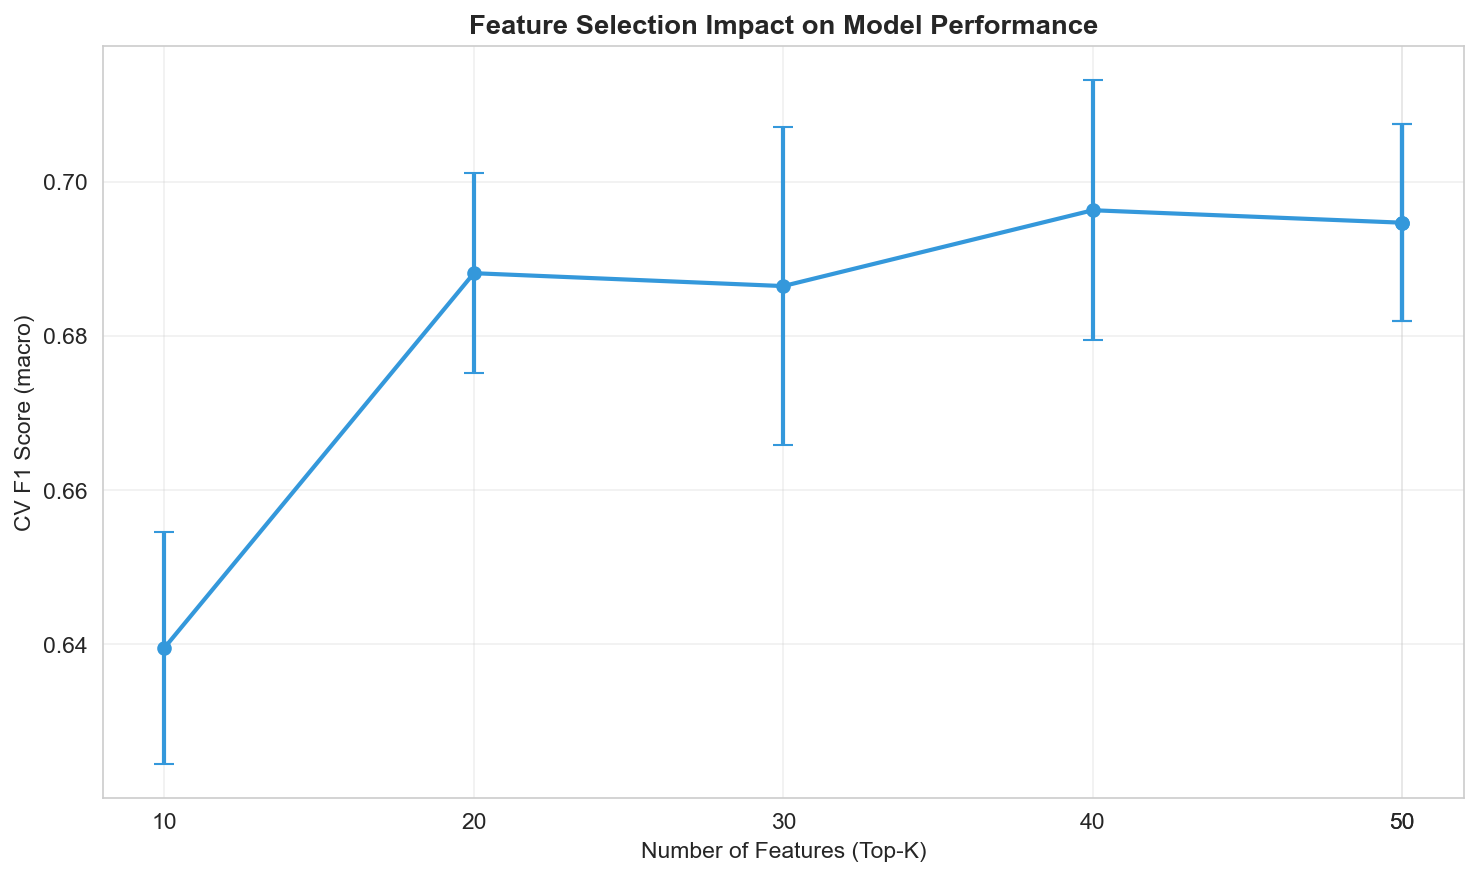
\includegraphics[width=\linewidth]{../data/plots/06_feature_selection_impact.png}
\caption{Feature count vs.\ CV F1 score.}
\label{fig:feature_selection}
\end{figure}

\begin{figure}[H]
\centering
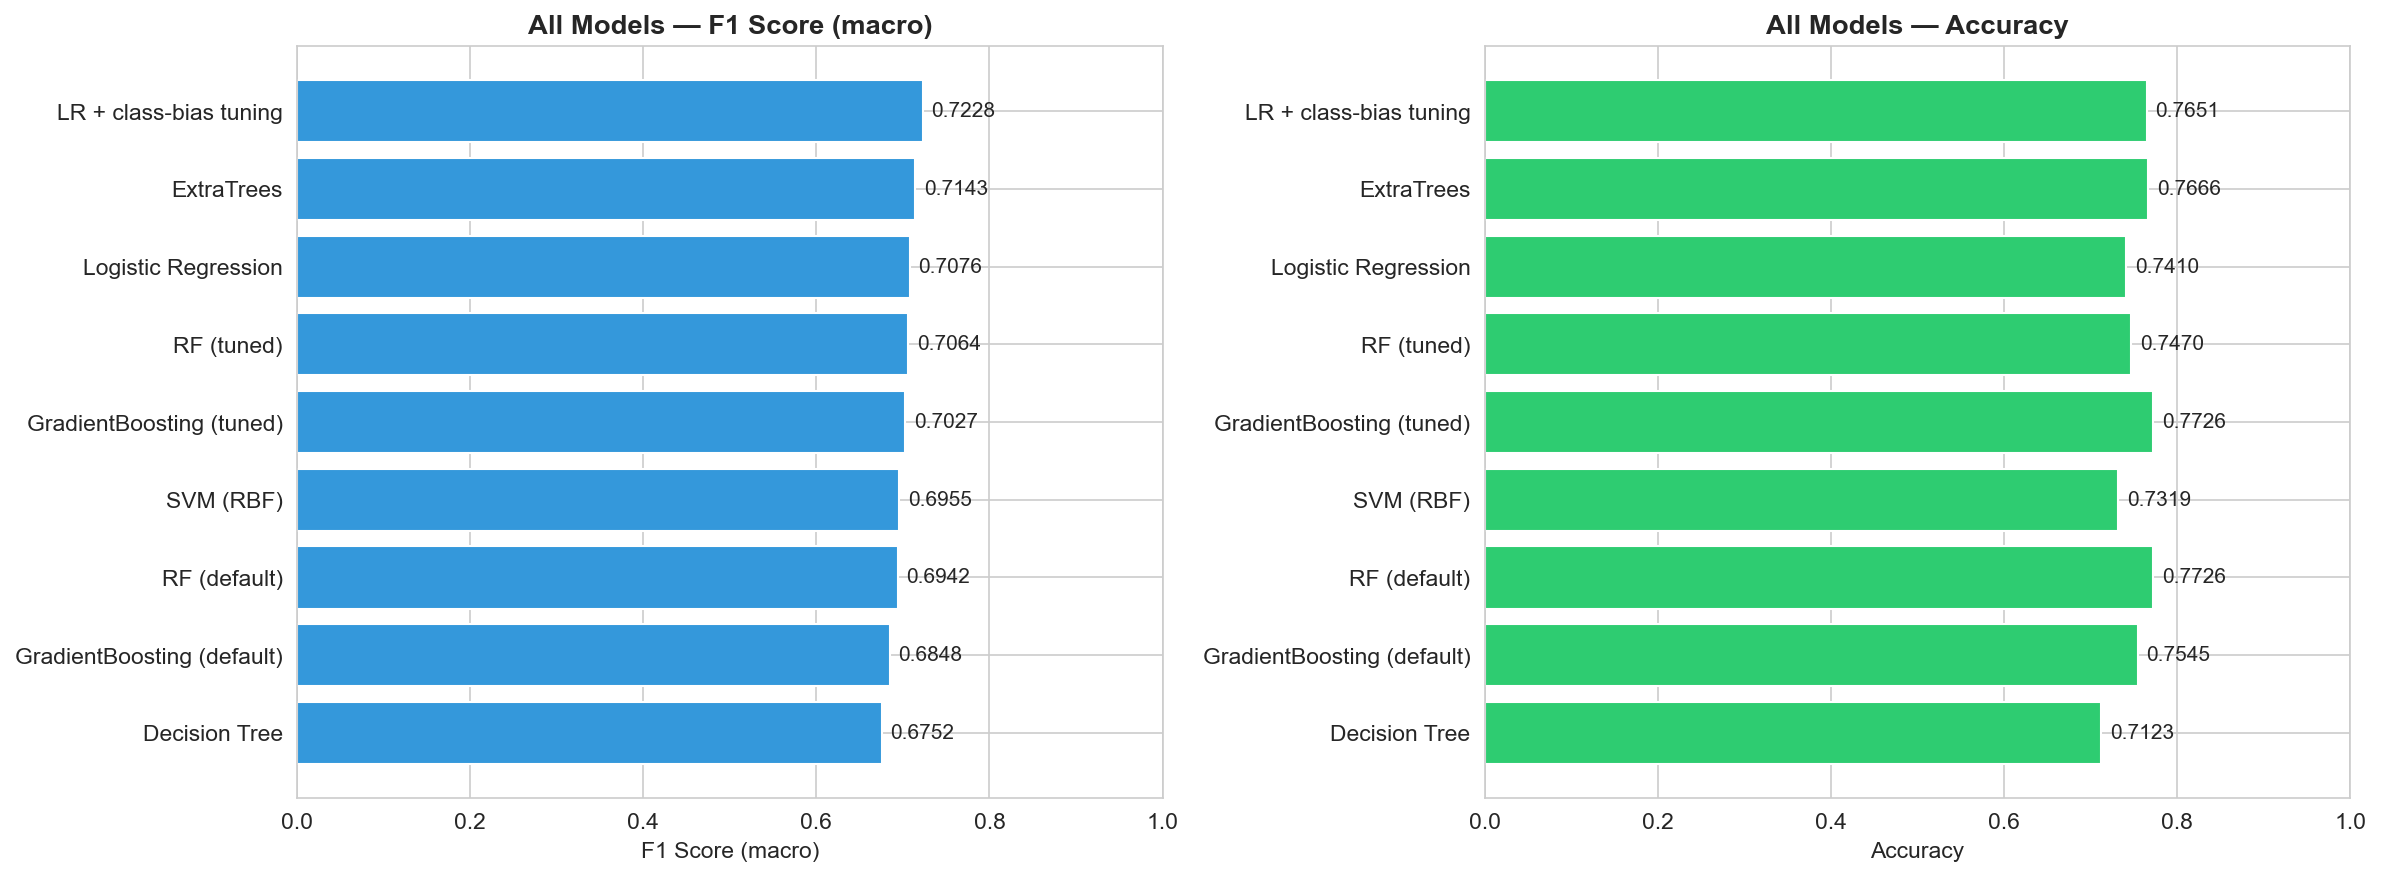
\includegraphics[width=\linewidth]{../data/plots/06_all_models_comparison.png}
\caption{Comprehensive comparison of all models --- F1 (macro) and accuracy.}
\label{fig:all_models_comparison}
\end{figure}

% ====================
\section{Conclusion}

Our analysis demonstrates that: (1) academic performance indicators (approval rates, grades) are the strongest predictors of student outcomes; (2) the ``Enrolled'' class is inherently ambiguous and represents the primary classification challenge; (3) hyperparameter tuning via validation curves effectively reduces overfitting, especially for Decision Trees; (4) ensemble methods provide the best overall performance.

% ====================
\section{References}

\begin{enumerate}
\item Realinho, V., et al. (2022). Student Dropout and Academic Success. UCI Machine Learning Repository. \url{https://doi.org/10.24432/C5MC89}
\item Pedregosa, F., et al. (2011). Scikit-learn: Machine Learning in Python. JMLR, 12, pp. 2825--2830.
\item Van der Maaten, L. and Hinton, G. (2008). Visualizing Data using t-SNE. JMLR, 9, pp. 2579--2605.
\end{enumerate}

% ====================
\section{Credit}

\subsection*{Group Member Contributions}

\begin{tabular}{ll}
\toprule
Member & Contribution \\
\midrule
[Member A] & [Data preprocessing, feature engineering] \\
[Member B] & [Clustering analysis, t-SNE visualization] \\
[Member C] & [Model training, evaluation, report writing] \\
[Member D] & [Open-ended exploration, presentation] \\
\bottomrule
\end{tabular}

\subsection*{GenAI Tools Disclosure}

This project used Claude by Anthropic (Claude 4 Opus) for the following support tasks:
\begin{itemize}
\item Code debugging and troubleshooting ($\sim$X\% of total coding effort)
\item Visualization code generation assistance ($\sim$X\%)
\item Report drafting and language polishing ($\sim$X\%)
\end{itemize}

All core machine learning implementations (data preprocessing, feature engineering, model training, hyperparameter tuning, and analysis) are the original work of group members. GenAI assistance accounted for less than 30\% of total project effort, in compliance with course policy.

\end{document}
